\documentclass[a4paper,fleqn]{cas-sc}
\usepackage[pagewise]{lineno}
\linenumbers

\usepackage[numbers]{natbib}
\usepackage[version=4]{mhchem}
\usepackage{array}
\usepackage{mathtools} 
\usepackage{tabularx}
\usepackage{booktabs}
\usepackage{threeparttable}
\usepackage{microtype}
\usepackage{xurl}
\usepackage{xcolor}
\usepackage{tikz}
\usetikzlibrary{arrows.meta,positioning,calc,fit,backgrounds}
\definecolor{cseBlue}{HTML}{0072B2}
\definecolor{cseOrange}{HTML}{D55E00}
\definecolor{cseSky}{HTML}{56B4E9}
\definecolor{cseInk}{HTML}{1F2933}

\tikzset{
  cse stage/.style={
    draw=cseBlue,
    fill=cseBlue!9,
    text=cseInk,
    rounded corners=2pt,
    align=center,
    minimum width=43mm,
    minimum height=10mm,
    inner sep=3pt,
    font=\small\bfseries,
  },
  cse detail/.style={
    draw=cseSky!75!black,
    fill=cseSky!7,
    text=cseInk,
    rounded corners=2pt,
    align=left,
    text width=67mm,
    minimum height=10mm,
    inner sep=4pt,
    font=\small,
  },
  cse solver/.style={
    draw=cseOrange,
    fill=cseOrange!8,
    text=cseInk,
    rounded corners=2pt,
    align=center,
    minimum width=43mm,
    minimum height=10mm,
    inner sep=3pt,
    font=\small\bfseries,
  },
  cse arrow/.style={-{Latex[length=2.2mm,width=1.5mm]},semithick,cseInk},
  cse link/.style={-{Latex[length=2mm,width=1.4mm]},semithick,cseBlue!80!black},
  cse region/.style={draw=cseBlue!40,fill=cseBlue!2,rounded corners=3pt,inner sep=4mm},
}

\newcolumntype{P}[1]{>{\centering\arraybackslash}p{#1}}
\newcommand{\Ha}{\text{Ha}}
\newcommand{\COtwo}{{\ce{CO2}}}
\newcommand{\HtwoO}{{\ce{H2O}}}
\newcommand{\MEA}{{\ce{MEA}}}
\newcommand{\MEAH}{\ce{MEAH+}}
\newcommand{\MEACOO}{{\ce{MEACOO-}}}
\newcommand{\HCOthree}{{\ce{HCO3-}}}
\newcommand{\Ntwo}{{\ce{N2}}}
\newcommand{\Otwo}{{\ce{O2}}}
\newcommand{\NtwoO}{{\ce{N2O}}}

\newcommand{\A}{\text{A}}
\newcommand{\B}{\text{B}}
\newcommand{\C}{\text{C}}
\newcommand{\D}{\text{D}}

\newcommand{\liq}{\ell}
\newcommand{\vap}{v}
\usepackage{placeins}

\usepackage{siunitx}
\usepackage{derivative}
\usepackage[nameinlink,noabbrev]{cleveref}
% Semantic notation used by the governing-equation layer.  The aliases keep
% the CAS manuscript's symbols while making phase and state roles explicit.
\newcommand{\differential}{\mathop{}\!\mathrm{d}}
\newcommand{\pressure}{P}
\newcommand{\temperature}{T}
\newcommand{\molarflow}{F}
\newcommand{\enthalpyflow}{\dot{H}}
\newcommand{\molarflux}{N}
\sisetup{detect-all,per-mode=symbol,range-phrase={--},range-units=single}
% CAS uses T1 fonts under XeLaTeX; select the degree glyph explicitly.
\DeclareSIUnit{\degreeCelsius}{\TextOrMath{\textdegree}{{}^{\circ}}C}
\Urlmuskip=0mu plus 2mu\relax
\AtBeginEnvironment{thebibliography}{\raggedright\sloppy\emergencystretch=3em}
% Suppress private exported notes without changing the Zotero bibliography.
\makeatletter
\providecommand{\bibinfo}[2]{#2}
\AtBeginEnvironment{thebibliography}{%
  \renewcommand{\bibinfo}[2]{\ifstrequal{#1}{note}{\unskip\@ifnextchar.{\@gobble}{}}{#2}}}
\makeatother

\begin{document}

    \def\floatpagepagefraction{1}
    \def\textpagefraction{.001}

    \shorttitle{Reactive ePC-SAFT for MEA Absorption}
    \shortauthors{T. W. Polley and J. D. Hedengren}

    % Main title of the paper
    \title[mode = title]{Reactive ePC-SAFT Modeling of Carbon Dioxide Absorption in Aqueous MEA}

    % Article type for Editorial Manager: Original Research Article.
    \author[1]{Tanner W. Polley}[orcid=0009-0008-5957-4152]
    \ead{tpolley3@byu.edu}

    \author[1]{John D. Hedengren}
    \cormark[1]
    \ead{john_hedengren@byu.edu}

    \affiliation[1]{
        organization={Department of Chemical Engineering, Brigham Young University},
        city={Provo},
        state={UT},
        postcode={84602},
        country={United States}
    }

    \cortext[cor1]{Corresponding author.}

    % Here goes the abstract
    \begin{abstract}
Electrolyte perturbed-chain statistical associating fluid theory (ePC-SAFT) provides a molecular thermodynamic description of the reactive liquid that can be coupled directly to absorber performance.
In two steady aqueous monoethanolamine (MEA) column formulations, ePC-SAFT supplies every bulk-phase thermodynamic property: liquid and vapor density, phase enthalpies and heat capacities, phase and reaction equilibrium among nine liquid species, \COtwo{} solubility, water fugacity and inlet water saturation; surface tension, transport, kinetics and packing performance remain correlations.
No thermodynamic parameter is fitted to the seven National Carbon Capture Center (NCCC) cases used for comparison.
A twelve-state conserved formulation with a finite-rate reactive film predicts capture with a mean absolute error of \num{3.55} percentage points at 129 axial nodes, against \num{4.52} for an equilibrium-manifold film and \num{7.51} for conventional enhancement; an \NtwoO{}-analogy solubility gives \num{3.61} points.
Every film overpredicts Case 6C, Case 7C capture is not resolved with respect to the axial mesh, and calculated liquid temperatures exceed the Case 7C packing temperatures by up to \qty{24}{K}.
A nine-species boundary-value-problem (BVP) formulation with conventional enhancement overpredicts all seven cases, with a mean absolute error of \num{5.86} points; its refined Case 3C capture is \qty{92.91}{\percent} versus \qty{89.50}{\percent} observed, mesh refinement changes it by \num{0.005} points, and one coarse solution takes about \qty{17}{s} of BVP wall time.
In that formulation the tested \(\pm5\%\) thermodynamic and \(\pm10\%\) transport changes affect capture by at most \num{0.8} and \num{0.3} points, and lean loadings of 0.225 and 0.275 mol \COtwo{} per mol MEA change capture by \num{+2.41} and \num{-3.92} points relative to 0.25.
    \end{abstract}

    \begin{keywords}
        Post-combustion \COtwo{} capture \sep MEA absorption \sep Boundary-value problems \sep Reactive film \sep Sensitivity analysis \sep ePC-SAFT \sep Fugacity driving force
    \end{keywords}

    \maketitle

    \section{Introduction}\label{sec:introduction}
% I1: engineering question
Predicting \COtwo{} capture in an aqueous monoethanolamine (MEA) absorber requires the coupled effects of reaction, interphase transfer and heat release to be represented.
MEA provides an experimentally documented reference solvent for rate-based packed-column models \cite{Freguia2003,Mores2012,Zhang2009}.
Outlet capture measures the overall removal of \COtwo, whereas axial temperatures describe the accompanying thermal response.
Their joint interpretation is needed to assess how solvent and gas conditions affect absorber performance.

% I2: established absorber capabilities
Rate-based MEA models already couple chemistry, equilibrium, transport and energy balances to pilot-scale observations \cite{Razi2013,Chinen2018,Morgan2018,Morgan2020}.
The studies in \cref{tab:absorber-literature-comparison} include resolved liquid-film calculations, enhancement approximations and experimental evaluations over multiple operating conditions.

\begin{table}[pos=htbp]
\centering
\small
\caption{Representative published absorber studies and the evidence they report. VLE denotes vapor--liquid equilibrium; eNRTL is electrolyte nonrandom two-liquid. The comparison concerns absorber studies rather than thermodynamic model families.}
\label{tab:absorber-literature-comparison}
\begin{tabularx}{\textwidth}{@{}>{\raggedright\arraybackslash}p{0.15\textwidth}*{3}{>{\raggedright\arraybackslash}X}@{}}
\toprule
Study & Thermodynamics, chemistry and film treatment & Calibration and evaluation coverage & Numerical method and reported inputs \\
\midrule
Tobiesen et al.\ \cite{Tobiesen2007} & Activity-coefficient VLE/speciation; reactive penetration-film model compared with three enhancement approximations & Evaluation of twenty steady-state pilot periods with \qty{30}{\percent} MEA; material/energy balances and temperature profiles (Tables 1--4) & Collocation with finite-difference Jacobian, \(10^{-6}\) tolerances and 31/51-point comparison; correlations/data in appendices; FORTRAN implementation \\
\addlinespace
Zhang et al.\ \cite{Zhang2009} & Hilliard/eNRTL thermodynamics with reversible carbamate/bicarbonate kinetics; Maxwell--Stefan two-film model, five liquid-film points & Evaluation of forty-one pilot-run sets spanning flows, loading and packing; representative temperature profiles (Tables 5--6, Figs.\ 12--14) & Aspen RateSep; 20-stage reference and 10/20/30/50-stage comparison (Tables 17--19). reaction/operating inputs given \\
\addlinespace
Chinen et al.\ \cite{Chinen2018} & eNRTL-consistent reduced chemistry with liquid-film reactions in rate-based RadFrac; hydraulic and mass-transfer correlation selection & Wetted-wall and packed-tower fitting; separately evaluated Notz pilot data over \qtyrange{40}{90}{\percent} capture (Fig.\ 11) & Forty-five tower control volumes; parameter estimation with multiple starts. equations and fitted constants in article/SI \\
\addlinespace
Akula et al.\ \cite{Akula2021} & Reduced two-reaction bulk equilibrium/film kinetics with property correlations and general enhancement-factor treatment & Wetted-wall calibration; seven NCCC and Technology Centre Mongstad absorber/stripper comparisons (Figs.\ 6--8, Table 5) & IDAES/Pyomo, IPOPT, 20 finite elements, four-stage homotopy and approximately \qty{65}{s} CPU time; equations/data in SI and code link given \\
\addlinespace
Shahid et al.\ \cite{Shahid2019} & Peng--Robinson vapor plus Kent--Eisenberg liquid chemistry; loading-dependent fast/slow reaction sections and two-film enhancement & Evaluation of low-pressure pilot cases and \qty{50}{bar} structured-packing data, including axial profiles (Figs.\ 4--9) & MATLAB axial integration with guessed gas composition; correlations/constants in Tables 1--4 \\
\bottomrule
\end{tabularx}
\end{table}


% I3: physical nonideality and reaction equilibrium
A molecular equation of state (EOS) supplies physical nonideality, whereas reaction equilibrium determines the distribution among molecular and ionic species.
Electrolyte perturbed-chain statistical associating fluid theory (ePC-SAFT) represents molecular and ionic interactions through residual Helmholtz energy \cite{Gross2001,Cameretti2005,Bulow2021a}.
Coupling its activities to reaction constants gives bulk speciation, and its fugacity coefficients provide a \COtwo{} driving force for interphase transfer.
The same Helmholtz energy also gives phase densities, enthalpies and heat capacities, so one model can supply every bulk-phase thermodynamic property an absorber balance needs, while surface tension, the interfacial film, transport and packing remain separate closures.

% I4: physical parameter reuse and comparative rationale
Available thermodynamic approaches differ in their physical representation and parameter requirements (\cref{tab:thermodynamic-model-comparison}).
eNRTL represents liquid excess Gibbs energy, Kent--Eisenberg uses simplified activities with effective reaction constants, and the cubic-plus-association EOS (CPA) and ePC-SAFT include association contributions.
An attraction of ePC-SAFT is that component-level segment, association and ionic descriptions enter explicit physical contributions, while combining rules supply cross interactions from reusable component inputs.
This offers a route to reducing additional mixture-specific binary fitting when extending a thermodynamic description to new solvents.

\begin{table*}
    \centering
    \small
    \caption{Comparison of the structure and parameter requirements of thermodynamic approaches commonly used for reactive amine absorption.}
    \label{tab:thermodynamic-model-comparison}
    \begin{tabularx}{\textwidth}{>{\raggedright\arraybackslash}p{2.5cm}*{3}{>{\raggedright\arraybackslash}X}}
        \toprule
        \textbf{Approach} & \textbf{Thermodynamics and chemistry} & \textbf{Reusable inputs and calibration} & \textbf{Application and extension limits} \\
        \midrule
        Kent--Eisenberg & Simplified liquid activities with effective reaction constants; vapor nonideality may be supplied separately & Physical solubility and acid--base inputs can be retained; effective constants require solvent/range-specific calibration \cite{Shahid2019,Zhu2022} & Useful for correlated acid-gas loading; another amine or blend requires appropriate chemistry and recalibration, not an electrolyte-EOS substitution \\
        eNRTL & Excess Gibbs energy gives liquid activities; reaction equilibrium supplies speciation; temperature derivatives and standard states supply calorics & Component properties, published binary parameters and fixed defaults can be reused; remaining directional interactions and ion standard-state properties are calibrated \cite{Zhang2011,Akula2023a} & Aqueous electrolyte VLE, speciation and calorics; extensions require internally consistent species, interactions, reaction and reference-state data \\
        CPA & Cubic EOS plus association gives phase fugacities; explicit chemistry or pseudo-chemical association describes reaction & Component cubic/association parameters and combining rules are reusable; cross-association and binary corrections may need fitting \cite{Chen2023} & Physical/associating mixtures and reactive-solubility applications; a pseudo-reaction fit does not by itself define a full ionic reaction network for another solvent \\
        ePC-SAFT & Residual Helmholtz energy gives density, activities and fugacities; explicit reaction constants determine reactive speciation & Component, association, ionic and dielectric inputs with combining rules; selected binary and reaction coefficients may require calibration \cite{Cameretti2005,Bulow2021a} & Reactive electrolyte states with consistent species and standard states; extension also needs reaction constants and applicable ion/mixture inputs \\
        \bottomrule
    \end{tabularx}
\end{table*}

% I5: scientific value of connecting thermodynamics to column response
Column evaluation connects these thermodynamic choices to the quantities needed for absorber design: capture, axial temperature and response to operating conditions.
Bulk speciation and fugacity profiles expose how the reactive EOS supplies the driving force, comparison of interfacial film descriptions with the same bulk thermodynamics isolates the transfer model, and separate thermodynamic and transport perturbations show how each set of inputs affects the coupled prediction.
Comparisons with measured capture and packing temperatures then assess that connection at the process scale.
Together with numerical refinement and measured computational cost, this provides a basis for developing predictive transfer models and testing thermodynamic parameter reuse in process calculations.

% I6: objective and reading order
Two column models are evaluated against seven National Carbon Capture Center (NCCC) one-bed cases.
A twelve-state conserved model compares three liquid-film descriptions, one of them with two interfacial \COtwo{} solubilities, on four axial meshes and locates the minimum Case 3C solvent flow for \qty{90}{\percent} capture.
A nine-species boundary-value-problem (BVP) model with conventional reaction enhancement \cite{polleyReactiveEPCSAFTModeling2026}, evaluated here with ePC-SAFT bulk-phase properties, carries a paired Case 3C refinement, a property-source comparison, thermodynamic and transport sensitivity studies and discrete changes in solvent flow, lean loading and inlet temperature.
Computational cost is measured for the coarse nine-species Case 3C calculation.


    \section{Absorber and thermodynamic model}\label{sec:model-framework}
\subsection{Physical system and model structure}
% M1: physical domain
The model describes steady countercurrent absorption in one packed bed.
Vapor flows upward from $z=0$ to $z=H$, while lean solvent enters at $z=H$ and flows downward; $H$ is packed height and $A$ is column cross-sectional area.
The apparent liquid components are \COtwo, MEA and water, and the wet gas contains \COtwo, water, nitrogen and oxygen.
Only \COtwo{} and water transfer between phases.
Two models of this system are evaluated.
The nine-species model integrates the column balances at constant pressure and carries the sensitivity, operating and computational-cost studies.
The twelve-state model (\cref{subsec:twelve-state}) solves conserved cell balances with a hydraulic pressure drop and leads the capture and temperature comparison.

% M2: calculation sequence
At each axial position, reactive equilibrium and transport calculations supply the fluxes used in the column balances (\cref{fig:absorber-calculation-sequence,tab:thermodynamic-responsibility}).
ePC-SAFT supplies every bulk-phase thermodynamic property in these balances: phase and reaction equilibrium, liquid and vapor densities, phase enthalpies and heat capacities, and the \COtwo{} and water fugacities.
With the MEA parameter set of \cref{sec:selected-reactive-inputs}, liquid temperature, pressure and apparent composition determine bulk speciation, density, enthalpy and the liquid \COtwo{} and water fugacities.
A wet four-species PC-SAFT vapor with published parameters supplies the water fugacity coefficient, vapor density and vapor enthalpy, and a reduced neutral vapor composition supplies the vapor \COtwo{} fugacity coefficient.
Surface tension, viscosity, diffusivity, reaction kinetics and packing performance remain correlations, and the \NtwoO{}-analogy Henry correlation of \cref{sec:properties} only generates the starting profile.
These quantities enter conventional enhancement and transfer resistances, and the resulting material and enthalpy sources determine the phase-flow and temperature derivatives.

\begin{figure}[pos=htbp]
\centering
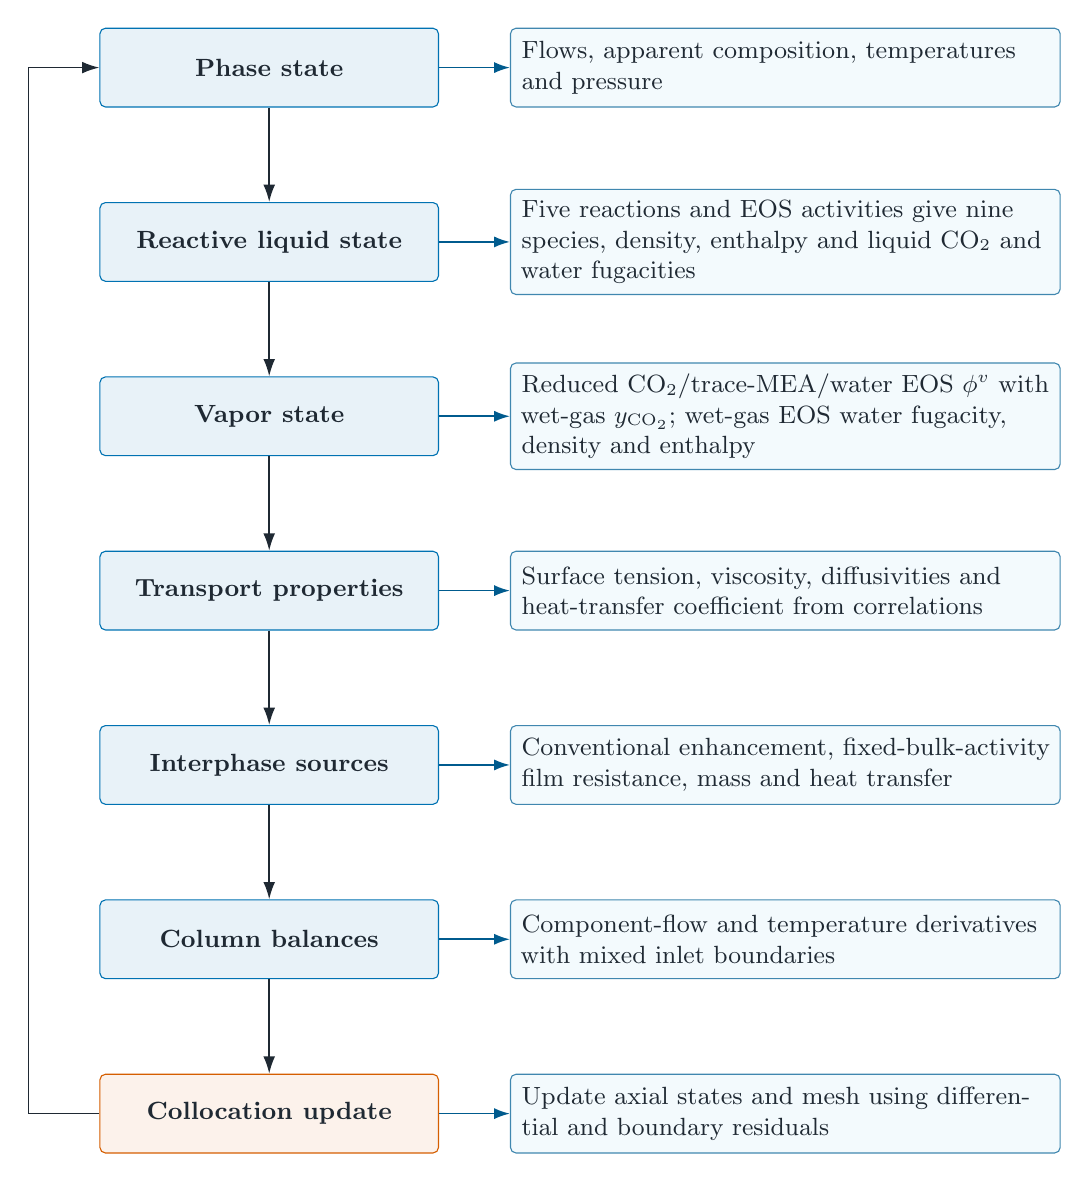
\begin{tikzpicture}[node distance=6mm and 9mm]
  \node[cse stage] (state) {Phase state};
  \node[cse detail,right=of state] (state-detail)
    {Flows, apparent composition, temperatures and pressure};
  \node[cse stage,below=12mm of state] (thermo) {Reactive liquid state};
  \node[cse detail,right=of thermo] (thermo-detail)
    {Five reactions and EOS activities give nine species, density, enthalpy and liquid CO$_2$ and water fugacities};
  \node[cse stage,below=12mm of thermo] (vapor) {Vapor state};
  \node[cse detail,right=of vapor] (vapor-detail)
    {Reduced CO$_2$/trace-MEA/water EOS $\phi^v$ with wet-gas $y_{\mathrm{CO_2}}$; wet-gas EOS water fugacity, density and enthalpy};
  \node[cse stage,below=12mm of vapor] (properties) {Transport properties};
  \node[cse detail,right=of properties] (properties-detail)
    {Surface tension, viscosity, diffusivities and heat-transfer coefficient from correlations};
  \node[cse stage,below=12mm of properties] (transport) {Interphase sources};
  \node[cse detail,right=of transport] (transport-detail)
    {Conventional enhancement, fixed-bulk-activity film resistance, mass and heat transfer};
  \node[cse stage,below=12mm of transport] (balances) {Column balances};
  \node[cse detail,right=of balances] (balances-detail)
    {Component-flow and temperature derivatives with mixed inlet boundaries};
  \node[cse solver,below=12mm of balances] (solver) {Collocation update};
  \node[cse detail,right=of solver] (solver-detail)
    {Update axial states and mesh using differential and boundary residuals};
  \foreach \from/\to in {state/thermo,thermo/vapor,vapor/properties,properties/transport,transport/balances,balances/solver}
    \draw[cse arrow] (\from) -- (\to);
  \foreach \name in {state,thermo,vapor,properties,transport,balances,solver}
    \draw[cse link] (\name.east) -- (\name-detail.west);
  \draw[cse arrow] (solver.west) -- ++(-9mm,0) |- (state.west);
\end{tikzpicture}

\caption{Coupled nine-species absorber calculation, from reactive speciation and phase driving forces through conventional enhancement and interphase sources to the column balances; feedback updates the axial state. A reduced CO$_2$/trace-MEA/water composition supplies the vapor CO$_2$ fugacity coefficient, and the wet four-species vapor supplies the water fugacity, density and enthalpy.}
\label{fig:absorber-calculation-sequence}
\end{figure}

\begin{table}[pos=htbp]
\centering\small
\caption{Quantities supplied by each part of the nine-species absorber model.}
\label{tab:thermodynamic-responsibility}
\begin{tabularx}{\textwidth}{@{}>{\raggedright\arraybackslash}p{0.24\textwidth}>{\raggedright\arraybackslash}X>{\raggedright\arraybackslash}X@{}}
\toprule
Calculation & Supplied quantities & Assumption or boundary \\
\midrule
Reactive liquid equilibrium and ePC-SAFT & Nine-species amounts, activities, density, enthalpy, apparent partial enthalpies and heat capacity; liquid CO$_2$ and water fugacities & Five reaction constants, conserved components and electroneutrality \\
Reduced neutral vapor EOS & CO$_2$ fugacity coefficient at total pressure & N$_2$/O$_2$ excluded from EOS composition; original wet-gas fraction used in $f^v=y_{\COtwo}\phi^vP$ \\
Wet four-species vapor PC-SAFT & Water fugacity coefficient, density, enthalpy, partial enthalpies and heat capacity; inlet water saturation & Published pure-component parameters, zero binary corrections and ideal-gas heat capacities \\
Enhancement-factor film & Enhancement and combined transfer resistance & $H_{\mathrm{bulk}}=f^\ell_{\COtwo}/C^{\ell,\mathrm{free}}_{\COtwo}$; bulk activity coefficient fixed across film \\
Correlations & Surface tension, viscosity, diffusivities, heat-transfer coefficient, kinetics and packing performance & Source ranges in \cref{tab:transport-applicability} \\
\bottomrule
\end{tabularx}
\end{table}

\subsection{Reactive equilibrium and phase driving forces}\label{subsec:thermodynamics}
% M3: species and conservation
Five reactions distribute the conserved apparent MEA--\COtwo--water composition among nine liquid species.
The liquid EOS and chemical-equilibrium equations are solved together at the liquid temperature and pressure of each axial position.
The nine true species, in the order used below, are \(\COtwo\), \(\MEA\), \(\HtwoO\), \(\MEAH\), \(\MEACOO\), \(\HCOthree\), \(\ce{CO3^{2-}}\), \(\ce{H3O+}\) and \(\ce{OH-}\).
The independent reactions are
\begin{align}
2\HtwoO &\rightleftharpoons \ce{H3O+}+\ce{OH-}, \tag{R1}\label{eq:reactive-r1}\\
\COtwo+2\HtwoO &\rightleftharpoons \HCOthree+\ce{H3O+}, \tag{R2}\label{eq:reactive-r2}\\
\HCOthree+\HtwoO &\rightleftharpoons \ce{CO3^{2-}}+\ce{H3O+}, \tag{R3}\label{eq:reactive-r3}\\
\MEACOO+\HtwoO &\rightleftharpoons \MEA+\HCOthree, \tag{R4}\label{eq:reactive-r4}\\
\MEAH+\HtwoO &\rightleftharpoons \MEA+\ce{H3O+}. \tag{R5}\label{eq:reactive-r5}
\end{align}
With products assigned positive stoichiometric coefficients, the equilibrium and conservation conditions are
\begin{align}
\sum_i\nu_{ir}\ln a_i^{\mathrm{EOS}}&=\ln K_r^{\mathrm{EOS}}(T,P),&
\mathbf B\mathbf n&=\mathbf B\mathbf n_0,\\
\mathbf M^{\mathsf T}\mathbf n&=\mathbf M^{\mathsf T}\mathbf n_0,&
\mathbf z^{\mathsf T}\mathbf n&=0.
\end{align}
Here \(\mathbf n\) contains true-species amounts, \(\mathbf n_0\) contains the apparent \(\COtwo\), MEA and water feed amounts with zero initial ionic amounts, \(\mathbf M\) contains formula-based molar masses, and \(\mathbf z=(0,0,0,1,-1,-1,-2,1,-1)^{\mathsf T}\).
The carbon and nitrogen balances use
\begin{equation}
\mathbf B=
\begin{bmatrix}
1&2&0&2&3&1&1&0&0\\
0&1&0&1&1&0&0&0&0
\end{bmatrix}.
\end{equation}
Mass conservation supplies the remaining independent composition constraint.

% M4: activities and standard states
Reaction equilibrium is evaluated on the molality activity basis with temperature-dependent constants.
The source standard state uses pure water and infinite-dilution solute molality, with \(m^\circ=\qty{1}{mol\,kg^{-1}}\).
Here $m_i^{\mathrm{mol}}$ is solute molality in moles per kilogram of solvent and $\gamma_i^{(m)}$ is its dimensionless molality-basis activity coefficient.
Source-basis solute activities are \(a_i^{\mathrm{src}}=\gamma_i^{(m)}m_i^{\mathrm{mol}}/m^\circ\); water uses its pure-solvent reference.
Reaction constants and chemical potentials are converted consistently to the EOS reference convention used in the equilibrium equations above.
Hereafter $K_r$ denotes the effective $K_r^{\mathrm{EOS}}(T,P)$, including its pressure-dependent reference conversion; temperature dependence is discussed at the fixed pressure of each column calculation.
\Cref{sec:selected-reactive-inputs} distinguishes the temperature correlations from these EOS-basis constants.

All five constants are fixed literature correlations on their source bases: R1--R3 from Austgen et al.\ \cite{Austgen1991}, R4 from Tong et al.\ \cite{Tong2012} and R5 from Bates and Pinching \cite{batesAcidicDissociationConstant1951}.
None was fitted with the parameter set.
The coefficients, source conventions and calculation domains are given in \cref{sec:selected-reactive-inputs}; their common temperature range is \qtyrange{293.15}{393.15}{K}.

The coupled liquid EOS supplies normalized true-species mole fractions and molar density, giving
\begin{equation}
C_i^{\mathrm{true}}=\rho_{\mathrm{EOS}}^{\liq}x_i^{\mathrm{true}}.
\end{equation}
These free and ionic concentrations enter reaction enhancement.
The same EOS density supplies the hydraulic calculation and the apparent-MEA concentrations used for diffusivity.


% M5: EOS physical contributions
The residual Helmholtz-energy model represents the physical interactions entering activities and fugacity coefficients.
For the liquid phase, the MEA electrolyte state activates the ionic terms.
In the vapor the same expressions apply without the electrolyte terms, because the vapor contains only neutral species.
For each phase state $(T,P,\mathbf{x})$, the EOS solves for the phase density and evaluates the residual Helmholtz energy as $\tilde{a}^{res}=\tilde{a}^{hc}+\tilde{a}^{disp}+\tilde{a}^{assoc}+\tilde{a}^{DH}+\tilde{a}^{Born}$.
The hard-chain term accounts for excluded-volume and chain-connectivity effects, the dispersion term accounts for attractive interactions, the association term accounts for site-specific association such as hydrogen bonding, the Debye--H\"uckel term accounts for long-range ionic screening, and the Born term accounts for ion-solvation work.
The five contributions are
\begin{align}
\tilde{a}^{hc}
&= \bar{m}\tilde{a}^{hs}
-\sum_i x_i(m_i-1)\ln g_{ii}^{hs}(\sigma_{ii})
&& \text{dimensionless}\label{eq:epcsaft-hc}\\
\tilde{a}^{disp}
&= -2\pi\widehat\rho I_1(\eta,\bar{m})\overline{m^2\epsilon\sigma^3}
-\pi\widehat\rho\bar{m}C_1I_2(\eta,\bar{m})\overline{m^2\epsilon^2\sigma^3}
&& \text{dimensionless}\label{eq:epcsaft-disp}\\
\tilde{a}^{assoc}
&= \sum_i x_i\sum_{A_i}
\left(\ln X^{A_i}-\frac{X^{A_i}}{2}+\frac{1}{2}\right)
&& \text{dimensionless}\label{eq:epcsaft-assoc}\\
\tilde{a}^{DH}
&=-\frac{\kappa e^{2}}{12\pi\varepsilon_{0}\varepsilon_{r,\mathrm{bulk}}k_{B}T}
\sum_i x_i z_i^2 \chi_i
&& \text{dimensionless}\label{eq:epcsaft-dh}\\
\tilde{a}^{Born}
&=
-\frac{e^2}{4\pi\varepsilon_0 k_B T}
\sum_i x_i z_i^2
\sum_{\delta\in\{\mathrm{bulk},\mathrm{ion}\}}
\left(1-\frac{1}{\varepsilon_{r,\delta}}\right)
D_i^{\delta}
&& \text{dimensionless}\label{eq:epcsaft-born}.
\end{align}
Here $m_i$ is the segment count of species $i$, $\bar{m}=\sum_i x_i m_i$ is the mean segment number and $\widehat\rho=10^{-30}N_A\rho_{\mathrm{mol}}$ is molecular number density in \unit{\angstrom^{-3}} when $\rho_{\mathrm{mol}}$ is in \unit{mol\,m^{-3}}.
The hard-sphere residual Helmholtz energy is $\tilde a^{hs}$, and $g_{ii}^{hs}$ is the hard-sphere contact radial distribution function.
The functions $I_1$ and $I_2$ are the first- and second-order dispersion integrals; $C_1$ is the hard-chain compressibility correction in the cited PC-SAFT formulation.
Pair diameters and energies obey $\sigma_{ij}=(\sigma_i+\sigma_j)/2$ and $\epsilon_{ij}=(1-k_{ij})\sqrt{\epsilon_i\epsilon_j}$.
The dispersion moments use segment diameters numerically in \unit{\angstrom} and reduced pair energies:
\begin{equation}
\overline{m^2\epsilon^n\sigma^3}
=\sum_i\sum_j x_i x_j m_i m_j
\left(\frac{\epsilon_{ij}/k_B}{T}\right)^n\sigma_{ij}^3,
\qquad n=1,2.
\end{equation}
Thus the density--moment products are dimensionless.
Further, $\eta$ is the packing fraction, $X^{A_i}$ is the fraction of nonbonded association sites, $\kappa$ is the inverse Debye screening length, and $\chi_i$ is the finite-ion-size screening factor.
The Born sum covers the bulk-solvent and ionic-shell regions, with relative permittivities $\varepsilon_{r,\delta}$ and reciprocal-diameter terms $D_i^{\delta}$ defined in \cref{sec:selected-reactive-inputs}.
The Born contribution follows Figiel et al.\ \cite{Figiel2025}, including its solvation-shell and dielectric-saturation (SSM+DS) terms.
The remaining auxiliary definitions, derivative expressions and mixing rules follow the cited PC-SAFT and ePC-SAFT formulations \cite{Gross2001,Cameretti2005,Bulow2019,Bulow2020,Bulow2021a}; the model choices and numerical inputs are given in \cref{sec:selected-reactive-inputs}.

% M6: actual phase driving forces
Interphase \COtwo{} transfer uses liquid fugacity from the reactive state and a vapor fugacity coefficient evaluated on a reduced neutral composition.
The vapor EOS excludes nitrogen and oxygen and normalizes CO$_2$, a numerical MEA trace and water:
\begin{align}
S_v&=\max(y_{\COtwo},\delta_x)+\delta_x+\max(y_{\HtwoO},\delta_x),\\
\widetilde{\mathbf y}&=\frac{1}{S_v}
\left(\max(y_{\COtwo},\delta_x),\delta_x,\max(y_{\HtwoO},\delta_x)\right),
\qquad\delta_x=10^{-12},\label{eq:reduced-vapor}\end{align}
where $\mathbf y$ is the full wet-gas composition and $\delta_x$ is a numerical MEA trace.
The coefficient evaluated at $T^\vap$, total pressure $P$ and $\widetilde{\mathbf y}$ is multiplied by the original wet-gas CO$_2$ fraction:
\begin{align}
f_{\COtwo}^{\vap}&=y_{\COtwo}\phi_{\COtwo}^{\vap}(T^\vap,P,\widetilde{\mathbf y})P,\\
f_{\COtwo}^{\liq}&=x_{\COtwo}^{\mathrm{true}}\phi_{\COtwo}^{\liq}(T^\liq,P,\mathbf x^{\mathrm{true}})P.
\label{eq:co2-fugacity}
\end{align}
Both fugacities are in pascals; the liquid fraction is the true-species mole fraction of unreacted molecular \COtwo{}, not apparent absorbed carbon.

Water fugacity is evaluated on the full phase compositions:
\begin{align}
f^{\:\vap}_{ \HtwoO} &= y_{\HtwoO}\phi^{\vap}_{\HtwoO}(T^\vap,P,\mathbf y)P && \left(\unit{Pa} \right)\\
f^{\:\liq}_{ \HtwoO} &= x^{\mathrm{true}}_{\HtwoO}\phi^{\liq}_{\HtwoO}(T^\liq,P,\mathbf x^{\mathrm{true}})P && \left(\unit{Pa} \right)
\end{align}
The liquid coefficient comes from the nine-species reactive state.
The vapor coefficient comes from a wet four-species PC-SAFT vapor of \COtwo{}, water, nitrogen and oxygen with published pure-component parameters \cite{Gross2001,Schick2023} and zero binary corrections; the same vapor state supplies vapor density, enthalpy and heat capacity.
The vapor--liquid fugacity difference supplies the driving force, while transfer coefficients, interfacial area and reaction enhancement determine the flux.

% M7: parameter origin
The liquid calculation uses the MEA parameter set of the authors' amine-thermodynamics study (\cref{sec:selected-reactive-inputs}).
Water, the two MEA-derived ions and their binary interactions were fitted jointly to vapor--liquid equilibrium, \COtwo{} solubility, speciation, absorption-heat, density and heat-capacity data; the remaining inputs are literature values or separate fits listed in \cref{sec:selected-reactive-inputs}.
No thermodynamic parameter was fitted to the NCCC cases, so the column comparisons are predictions of the parameter set.
Because liquid densities are in the fit objective, the density comparison of \cref{sec:properties} uses only rows outside it.
Ideal-gas heat capacities and formation enthalpies of \COtwo{} and water \cite{chaseNISTJANAFThermochemicalTables1998,internationalassociationforthepropertiesofwaterandsteamRevisedReleaseIAPWS2018} and of MEA \cite{Zhang2011} complete the caloric description of both phases.
Reaction enthalpies follow from the temperature derivatives of the five equilibrium constants.

\subsection{Hydraulics, transfer coefficients and enhancement}\label{subsec:transport}
% M8: hydraulic dependencies
Flows and mixture properties at each axial position determine phase velocities, liquid holdup and effective interfacial area.
The correlations below use the EOS phase densities together with viscosity, surface tension and diffusivity correlations on the bases in \cref{sec:properties}.
The hydraulic calculation requires positive properties and $0<h_L<\epsilon$, where $h_L$ and $\epsilon$ are liquid holdup and bed void fraction.
In the nine-species model a pressure-drop correlation is evaluated only to check the hydraulic operating range, and pressure is held constant in the balances.


\paragraph{Hydraulic quantities.}
The superficial velocities of each phase are calculated from molar flow rate, column area, and molar density:
\begin{align}
u^{\liq} &= \frac{\molarflow^{\liq}_{T}}{A \,\rho^{\liq}_{ \text{mol}}}
&& \left(\unit{m\,s^{-1}}\right)\\
u^{\vap} &= \frac{\molarflow^{\vap}_{T}}{A \,\rho^{\vap}_{ \text{mol}}}
&& \left(\unit{m\,s^{-1}}\right).
\end{align}


The effective interfacial area converts packed-bed geometry and liquid wetting into available transfer area per bed volume.
It depends on liquid density, surface tension, superficial velocity, and packing geometry.
The adopted expression follows the form reported by Tsai~\cite{Tsai2010}; \cref{tab:transport-applicability} compares its coefficients and source range.
\begin{align}
a_e
&= 1.42\,a_p\left[\frac{\rho^{\liq}}{\sigma^{\liq}}\,g^{1/3}\left(\frac{u^{\liq}\epsilon}{a_p}\right)^{4/3}\right]^{0.12} && \left(\unit{m^{-1}}\right)
\end{align}

Here \(\rho^{\liq}\) is liquid mass density, \(a_p\) is packing specific area and \(g\) is gravitational acceleration.


Liquid holdup, the liquid volume per packed-bed volume, enters the transfer-coefficient correlations of Chinen et al.\ and Tsai~\cite{Chinen2018,Tsai2010}:
\begin{align}
h_{L,\mathrm{raw}} &= 11.4474\left[3.185966\,u^{\liq}\left(\frac{\mu^{\liq}}{\rho_{\mathrm{mass}}^{\liq}}\right)^{1/3}\right]^{0.6471}
&& \text{dimensionless}\\
h_L &= \frac{\epsilon h_{L,\mathrm{raw}}}{\epsilon+h_{L,\mathrm{raw}}},&
h_V &= \epsilon-h_L.
\end{align}
The empirical coefficients use velocity in \unit{m\,s^{-1}}, viscosity in \unit{Pa\,s} and mass density in \unit{kg\,m^{-3}}.
The bounded mapping is applied to the raw correlation and ensures \(0<h_L<\epsilon\) for positive inputs.

\paragraph{Mass and heat transfer.}
% M9: mass and heat transfer
Gas- and liquid-side coefficients provide the physical resistances to interphase transfer.
Their correlations depend on phase density, viscosity, diffusivity, velocity and packing geometry.
The coefficients and constants follow regression-based packed-column correlations reported by Billet and Schultes and by Chinen and co-workers~\cite{Billet1999,Chinen2018}.
\begin{align}
k^{\liq}_i &= C_L
\left(\frac{g\rho^{\liq}}{\mu^{\liq}}\right)^{1/6}
\left(\frac{1}{d_h}\right)^{1/2}
\left(\frac{u^{\liq}}{a_p}\right)^{1/3}
{D_i^{\liq}}^{1/2}
&& \left(\unit{m\,s^{-1}}\right)\\
k^{\vap}_i &= \frac{C^{\vap}}{R\,T^{\vap}}
\left(\frac{a_p}{d_h\,h_V}\right)^{1/2}
\left(\frac{u^{\vap}\rho^{\vap}}{a_p\,\mu^{\vap}}\right)^{3 / 4}
{D_i^{\vap}}^{2 / 3}
\left(\frac{\mu^{\vap}}{\rho^{\vap}}\right)^{1 / 3}
&& \left(\unit{mol\,Pa^{-1}\,m^{-2}\,s^{-1}}\right)
\end{align}

Here \(d_h=4\epsilon/a_p\) is the hydraulic diameter; \(\rho^{\liq}\) and \(\rho^{\vap}\) are phase mass densities.
The adopted packing coefficients are \(C_L=0.203\) and \(C^{\vap}=0.35\).


The overall heat-transfer coefficient is estimated with the Chilton--Colburn analogy:
\begin{align}
U_T = \left(\frac{(k^{\vap}_{\COtwo}\,P)^3\,{k_{t}^{\vap}}^{2}\,C^{\vap}_{p,T}}{\left(\rho^{\vap}_{\text{mol}}D^{\vap}_{\COtwo}\right)^2}\right)^{\frac{1}{3}}
&& \left(\unit{J\,s^{-1}\,m^{-2}\,K^{-1}}\right)
\end{align}

\paragraph{Reaction enhancement.}
% M10: enhancement and film approximation
A conventional enhancement factor represents reaction-enhanced liquid-side \COtwo{} transfer as a ratio to physical absorption.
The adopted pseudo-second-order approximation follows the form of Gaspar and Fosb\o l \cite{Gaspar2015}, using bulk free-species concentrations without solving coupled reaction--diffusion equations in the liquid film.
The rate expression and Hatta number are
\begin{align}
k_{\MEA} &= 2.003\times10^4\exp(-4742.0/T^{\liq})
&& \left(\unit{m^6\,mol^{-2}\,s^{-1}}\right)\\
k_{\HtwoO} &= 4.147\exp(-3110/T^{\liq})
&& \left(\unit{m^6\,mol^{-2}\,s^{-1}}\right)\\
k_2 &= k_{\MEA}C^{\liq}_{\MEA,true}+k_{\HtwoO}C^{\liq}_{\HtwoO,true}
&& \left(\unit{m^3\,mol^{-1}\,s^{-1}}\right)\\
Ha &= \frac{\sqrt{k_2 C^{\liq}_{\MEA,true} D^{\liq}_{\COtwo}}}{k^{\liq}_{\COtwo}}
&& \text{dimensionless}
\end{align}
Here $k_2$ is the pseudo-second-order rate coefficient and $Ha$ compares the rate of reaction in the liquid film to diffusion through that film.
The enhancement calculation uses an effective dissolved-\COtwo{} concentration
$\widetilde C^{\liq}_{\COtwo}=C^{\liq}_{\COtwo,true}/s_{\COtwo}$, with the fixed dimensionless divisor
$s_{\COtwo}=1.0454$ (full precision in \cref{sec:selected-reactive-inputs}).
This empirical correction applies only within the enhancement calculation, not to species balances or EOS fugacity.
The dimensionless resistance terms are
\begin{align}
R_+ &= \frac{D^{\liq}_{\MEA} C^{\liq}_{\MEA,true}}
{2D^{\liq}_{\MEAH} C^{\liq}_{\MEAH,true}}
&& \text{dimensionless}\\
R_- &= \frac{D^{\liq}_{\MEA} C^{\liq}_{\MEA,true}}
{2D^{\liq}_{\MEACOO} C^{\liq}_{\MEACOO,true}}
&& \text{dimensionless}\\
\widehat{E} &= \frac{D^{\liq}_{\MEA} C^{\liq}_{\MEA,true}}
{2D^{\liq}_{\COtwo} \widetilde C^{\liq}_{\COtwo}}
&& \text{dimensionless}
\end{align}
which gives the explicit enhancement factor
\begin{align}
E &= 1+\frac{Ha-1}{1 + Ha(R_+ + R_- + 2)/\widehat{E}}
&& \text{dimensionless}.
\end{align}
Numerical evaluation bounds the denominators away from zero and restricts $E$ to $1\leq E\leq10^4$; the raw holdup correlation is bounded at \(10^{-12}\epsilon\).

The conventional two-film approximation relates interfacial fugacity to free molecular concentration with the bulk activity coefficient held fixed across the liquid film:
\begin{equation}
H_{\mathrm{bulk}}=\frac{f^{\ell}_{\COtwo}}{C^{\ell,\mathrm{free}}_{\COtwo}},
\qquad \Psi_H=\frac{E k^{\ell}_{\COtwo}}{E k^{\ell}_{\COtwo}+k^{v}_{\COtwo}H_{\mathrm{bulk}}}.
\end{equation}
The coefficient $H_{\mathrm{bulk}}$, the ePC-SAFT Henry coefficient below, has units of \unit{Pa\,m^3\,mol^{-1}} and uses fugacity and free \COtwo{} concentration from the same bulk equilibrium state.
Bulk equilibrium determines the liquid state, while enhancement approximates film chemistry.
\Cref{tab:transport-applicability} gives the source ranges of these correlations; \cref{sec:results} compares them with the calculated states.

% M11: flux construction
\paragraph{Interphase sources.}
The interphase molar source per unit packed length determines how $\COtwo$ and $\HtwoO$ transfer between phases along the packed height.
\begin{align}
\molarflux^{\vap}_{ \COtwo} &=  -k^{\vap}_{ \COtwo}  a_e A  \left(f^{\:\vap}_{ \COtwo} - f^{\:\liq}_{ \COtwo}\right) \Psi _{H} && \left(\unit{mol\,s^{-1}\,m^{-1}}\right) \\
\molarflux^{\liq}_{ \COtwo} &= -\molarflux^{\vap}_{ \COtwo} && \left(\unit{mol\,s^{-1}\,m^{-1}}\right) \\
\molarflux^{\vap}_{ \HtwoO} &= -k^{\vap}_{ \HtwoO} a_e A \left(f^{\:\vap}_{ \HtwoO} - f^{\:\liq}_{ \HtwoO}\right)  && \left(\unit{mol\,s^{-1}\,m^{-1}}\right) \\
\molarflux^{\liq}_{ \HtwoO} &= -\molarflux^{\vap}_{ \HtwoO} && \left(\unit{mol\,s^{-1}\,m^{-1}}\right)
\end{align}
Here $N_i^j$ is an interphase source per unit packed length, in \unit{mol.s^{-1}.m^{-1}}.
Positive $f_i^v-f_i^\ell$ gives a negative vapor source and an equal positive liquid source.
The area $a_eA$ converts interfacial transfer per area into this axial source; changes in the phase state recalculate its driving force, coefficients and enhancement.


The interphase enthalpy source contains the enthalpy carried by transferred \COtwo{} and \HtwoO{} plus sensible heat exchange between phases.
Heat transfer is modeled with the same effective interfacial area and the overall heat-transfer coefficient $U_T$:
\begin{align}
q^{\vap} &= -U_T a_e A \left(T^{\vap}-T^{\liq}\right) && \left(\unit{J\,s^{-1}\,m^{-1}}\right) \\
q^{\liq} &= -U_T a_e A \left(T^{\liq}-T^{\vap}\right) && \left(\unit{J\,s^{-1}\,m^{-1}}\right) \\
\enthalpyflow^{\vap}_{flux} &=   \molarflux^{\vap}_{ \COtwo}H^{\vap}_{ \COtwo} + \molarflux^{\vap}_{ \HtwoO}H^{\vap}_{ \HtwoO} +  q^{\vap} && \left(\unit{J\,s^{-1}\,m^{-1}}\right) \\
\enthalpyflow^{\liq}_{flux} &= -\left(\molarflux^{\vap}_{ \COtwo}H^{\vap}_{ \COtwo} + \molarflux^{\vap}_{ \HtwoO}H^{\vap}_{ \HtwoO}\right) +  q^{\liq} && \left(\unit{J\,s^{-1}\,m^{-1}}\right)
\end{align}

Here $H^{\vap}_i$ is the partial molar enthalpy of component $i$ in the wet vapor at $T^\vap$, so transferred \COtwo{} and water carry vapor-phase enthalpy across the interface.
The liquid-side enthalpy source is written as the negative vapor-side transferred enthalpy plus heat transfer so that interphase enthalpy transfer is conservative.
The heat of absorption therefore appears through the difference between these vapor partial enthalpies and the liquid partial enthalpies in the temperature equation below.

\subsection{Column balances and boundary conditions}\label{subsec:governing-equations}
\subsubsection{Material balance}\label{subsubsec:material-balance}
% M12: material conservation
Phase component flows change through the interfacial sources with signs set by the countercurrent coordinate.
Only \COtwo{} and \HtwoO{} transfer between phases; their component balances are
\begin{align}
\odv{\molarflow^{\liq}_{ \COtwo}}{z} &= -\molarflux^{\liq}_{ \COtwo} + \delta_F && \left(\unit{mol\,s^{-1}\,m^{-1}}\right)\\
\odv{\molarflow^{\liq}_{ \HtwoO}}{z} &= -\molarflux^{\liq}_{ \HtwoO} + \delta_F && \left(\unit{mol\,s^{-1}\,m^{-1}}\right)\\
\odv{\molarflow^{\vap}_{ \COtwo}}{z} &= \molarflux^{\vap}_{ \COtwo} + \delta_F && \left(\unit{mol\,s^{-1}\,m^{-1}}\right)\\
\odv{\molarflow^{\vap}_{ \HtwoO}}{z} &= \molarflux^{\vap}_{ \HtwoO} + \delta_F && \left(\unit{mol\,s^{-1}\,m^{-1}}\right)\label{eq:material-balance}
\end{align}
The evaluated flow equations include the common numerical offset \(\delta_F=\qty{1e-10}{mol\,s^{-1}\,m^{-1}}\).
It is retained in the temperature chain rule and cancels in the signed countercurrent component balance, \(\odv{(\molarflow_i^\vap-\molarflow_i^\liq)}{z}=0\).
MEA, \Ntwo, and \Otwo{} are treated as non-transferring apparent components over the one-bed calculation.
Phase compositions and loading are reconstructed from the solved flow variables:
\begin{align}
x_i &= \frac{\molarflow^{\liq}_{ i}}{\molarflow^{\liq}_{ T}}
&& \text{dimensionless}\\
y_i &= \frac{\molarflow^{\vap}_{ i}}{\molarflow^{\vap}_{ T}}
&& \text{dimensionless}\\
\alpha &= \frac{x_{\COtwo}}{x_{\MEA}}
&& \text{dimensionless}
\end{align}

\subsubsection{Energy balance}\label{subsubsec:energy-balance}
% M13: continuous energy equations
Nonisothermal balances use the ePC-SAFT phase enthalpies and the heat-transfer expression above.
Interphase heat and material transfer supply the enthalpy-flow derivatives:
\begin{align}
\odv{\enthalpyflow^{\liq}}{z} &= -\enthalpyflow^{\liq}_{flux} && \left(\unit{J\,s^{-1}\,m^{-1}}\right)\\
\odv{\enthalpyflow^{\vap}}{z} &= \enthalpyflow^{\vap}_{flux} && \left(\unit{J\,s^{-1}\,m^{-1}}\right)\label{eq:energy-balance}
\end{align}
The liquid sign follows its flow opposite increasing $z$, so the continuous equations give $\odv{(\enthalpyflow^{\vap}-\enthalpyflow^{\liq})}{z}=0$.
The liquid enthalpy flow is the enthalpy of the reacting nine-species liquid at fixed apparent \COtwo{}, MEA and water amounts, so speciation shifts with temperature and composition are included.
The vapor enthalpy flow is that of the wet four-species vapor.
With apparent partial molar enthalpies $H_i^j=(\partial\enthalpyflow^j/\partial\molarflow_i^j)_{T,P}$ of the phase-$j$ components, the temperature chain rule is
\begin{align}
\odv{\temperature^j}{z} &= \frac{\odv{\enthalpyflow^j}{z} - \sum_i H_i^j\odv{\molarflow_i^j}{z}}{\molarflow^j \left(\pdv{H^j}{\temperature^j}\right)_{P,\boldsymbol{x}^j}}
&& \left(\unit{K\,m^{-1}}\right)
\end{align}
For the transferring components \(\mathcal T=\{\COtwo,\HtwoO\}\), substitution gives
\begin{align}
\odv{\temperature^\liq}{z}
&=\frac{-\enthalpyflow^\liq_{flux}+\sum_{i\in\mathcal T}H_i^\liq(\molarflux_i^\liq-\delta_F)}
{\molarflow^\liq(\partial H_T^\liq/\partial T^\liq)_{\boldsymbol{x}}}
&&\left(\unit{K\,m^{-1}}\right),\\
\odv{\temperature^\vap}{z}
&=\frac{\enthalpyflow^\vap_{flux}-\sum_{i\in\mathcal T}H_i^\vap(\molarflux_i^\vap+\delta_F)}
{\molarflow^\vap C_{p,T}^\vap}
&&\left(\unit{K\,m^{-1}}\right).
\end{align}
At fixed apparent composition, the vapor derivative is the wet-gas heat capacity $C_{p,T}^{\vap}$ and the liquid derivative is the heat capacity of the reacting liquid, including the enthalpy of the speciation shift with temperature.
The ePC-SAFT calculation supplies both enthalpies, their partial enthalpies and their temperature derivatives from the residual Helmholtz energy and the ideal-gas records.
Numerical variation of the net enthalpy flow is measured separately in \cref{eq:energy-range}.

\subsubsection{State vector and pressure}
% M14: differential states
The differential state comprises four transferring component flows, two phase temperatures and pressure.
The nine-species model holds pressure constant over the bed:
\begin{align}
\odv{\pressure}{z} = 0
&& \left(\unit{Pa\,m^{-1}}\right).
\end{align}

The differential state vector used for the coupled calculations and its derivative mapping are given in \cref{eq:state-vector,eq:state-derivative}:
\begin{align}
\mathbf{y}(z) &=
\begin{pmatrix}
\molarflow^{\liq}_{\COtwo}(z)\\[4pt]
\molarflow^{\liq}_{\HtwoO}(z)\\[4pt]
\molarflow^{\vap}_{\COtwo}(z)\\[4pt]
\molarflow^{\vap}_{\HtwoO}(z)\\[4pt]
\temperature^{\liq}(z)\\[4pt]
\temperature^{\vap}(z)\\[4pt]
\pressure(z)
\end{pmatrix}
&& \left(
4\times\unit{mol\,s^{-1}},
2\times\unit{K},
\unit{Pa}
\right)^{\mathsf{T}}\label{eq:state-vector},\\[1em]
\odv{\mathbf{y}}{z} &=
\begin{pmatrix}
\odv{\molarflow^{\liq}_{ \COtwo}}{z} \\[4pt]
\odv{\molarflow^{\liq}_{ \HtwoO}}{z} \\[4pt]
\odv{\molarflow^{\vap}_{ \COtwo}}{z} \\[4pt]
\odv{\molarflow^{\vap}_{ \HtwoO}}{z} \\[4pt]
\odv{\temperature^{\liq}}{z} \\[4pt]
\odv{\temperature^{\vap}}{z}\\[4pt]
\odv{\pressure}{z}
\end{pmatrix}
\equiv
\mathbf{f}(z, \mathbf{y})
&& \left(
4\times\unit{mol\,s^{-1}\,m^{-1}},
2\times\unit{K\,m^{-1}},
\unit{Pa\,m^{-1}}
\right)^{\mathsf{T}}.\label{eq:state-derivative}
\end{align}
The dimensional coordinate is $z\in[0,H]$.
For normalized height $\zeta=z/H$, the solver uses $d\mathbf y/d\zeta=H\mathbf f$; figures display this normalized coordinate.

\subsubsection{Boundary conditions}
% M15: mixed boundaries
Gas-inlet and liquid-inlet specifications define mixed boundary conditions because the phases enter at opposite ends.
Let $a=0$ denote the vapor inlet and $b=H$ denote the liquid inlet.
The temperature-state calculation requires seven inlet boundary conditions:
\begin{align}
\boldsymbol{\alpha} &= \left[\molarflow^{\vap}_{ \COtwo, a}, \molarflow^{\vap}_{ \HtwoO, a}, \temperature^{\vap}_{ a}, \pressure_{a}\right]
&& \left(
2\times\unit{mol\,s^{-1}},
\unit{K},
\unit{Pa}
\right)^{\mathsf{T}}\label{eq:boundary-conditions}\\
\boldsymbol{\beta} &= \left[\molarflow^{\liq}_{ \COtwo, b}, \molarflow^{\liq}_{ \HtwoO, b}, \temperature^{\liq}_{ b}\right]
&& \left(
2\times\unit{mol\,s^{-1}},
\unit{K}
\right)^{\mathsf{T}}
\end{align}
or equivalently, the boundary residual is
\begin{align}
\mathbf{r}(\mathbf{y}) &=
\begin{pmatrix}
\mathbf{y}_{\vap}(a)-\boldsymbol{\alpha}\\
\mathbf{y}_{\liq}(b)-\boldsymbol{\beta}
\end{pmatrix}
=
\mathbf{0}
&& \left(
2\times\unit{mol\,s^{-1}},
\unit{K},
\unit{Pa},
2\times\unit{mol\,s^{-1}},
\unit{K}
\right)^{\mathsf{T}}.\label{eq:boundary-residual}
\end{align}

The specified gas flows are reconstructed from reported dry inputs and water vapor saturated at the gas-inlet temperature and pressure, while liquid flows follow reported mass flow, solvent composition and lean loading.
Saturation solves equality of the vapor water fugacity with that of pure liquid water at fixed dry-gas proportions, with both phases evaluated by the same PC-SAFT water parameters.
MEA and inert-gas flows remain constant, and the outlet transferring flows and phase temperatures are calculated rather than imposed.

\subsection{Twelve-state conserved model}\label{subsec:twelve-state}
% M16: twelve-state states and balances
The twelve-state model writes the same countercurrent bed as conservative cell balances solved simultaneously at all axial nodes.
Its states at each node are four apparent component flows, the liquid and gas temperatures, pressure, liquid holdup, the \COtwo{} and water interphase fluxes, the total energy flux and the interface log-loading.
Seven conserved balances and five algebraic relations close these states.
Seven boundary equations specify the gas inlet at the bottom and the liquid inlet at the top.
The phase enthalpies are the ePC-SAFT total enthalpies, the liquid density is the density of the solved reactive state, and pressure falls along the bed through a hydraulic pressure-drop correlation.

% M17: twelve-state film descriptions
Three descriptions of the liquid film are compared within this model.
The finite-rate film combines the film conductance along the equilibrium manifold at each axial position with a kinetic resistance from a Hatta-number film solution, using the rate expression of \cref{subsec:transport}.
Its interfacial \COtwo{} solubility is either the ePC-SAFT Henry coefficient $H_{\mathrm{bulk}}$ or the \NtwoO{}-analogy Henry coefficient of \cref{sec:properties}, which gives four film variants.
The equilibrium-manifold film assumes chemical equilibrium throughout the film, and the enhancement-factor film uses the conventional enhancement factor of \cref{subsec:transport}.
All three use nine-point film quadrature.

% M18: twelve-state input basis
The twelve-state inputs differ from the nine-species inputs.
They read the reported gas mass flow as wet gas, set the inlet water content from a pure-water vapor-pressure correlation and start from the reported gas-inlet pressure.
In Case 3C the twelve-state dry-gas flow is therefore about \qty{5}{\percent} lower than the nine-species value.
Its gas phase uses a separate four-species PC-SAFT parameter set, with a \COtwo{} dispersion energy of \qty{173.44}{K} and a constant \COtwo--water $k_{ij}$ of \num{0.01326}, instead of the published parameters of the nine-species vapor.
Capture differences between the two models therefore combine differences in model structure and inputs.


    \section{Evaluation methods}\label{sec:methods}
\subsection{Experimental cases and reported quantities}
% E1: comparison inputs
Seven one-bed, no-intercooler cases from the 2017 NCCC C campaign provide the experimental comparison \cite{Morgan2020}.
The modeled bed has diameter \qty{0.64}{m}, height \qty{6}{m} and MellapakPlus 252Y packing, with specific area \qty{250}{m^{-1}} and void fraction 0.970.
\Cref{tab:nccc-one-bed-scope} gives the reported operating inputs; the missing lean-inlet temperatures in Cases 1C--3C are set to \qty{318.15}{K}.
In the nine-species model, reported dry gas mass flow and dry \COtwo{} fraction are converted to a wet feed by PC-SAFT water saturation at the gas-inlet temperature and pressure, with the remaining dry gas distributed between nitrogen and oxygen using $y_{\Otwo}/y_{\Ntwo}=0.08485753604$.
These inputs apply to the nine-species comparison and to the Case 3C reference used below; the twelve-state input basis is given in \cref{subsec:twelve-state}.

\begin{table}[pos=htbp]
  \centering
  \footnotesize
  \caption{Reported and assumed inputs and reported capture for the seven NCCC one-bed, no-intercooler cases \cite{Morgan2020}.}
  \label{tab:nccc-one-bed-scope}
  \begin{threeparttable}
  \setlength{\tabcolsep}{2.5pt}
  \begin{tabular*}{\textwidth}{@{\extracolsep{\fill}}ll
    S[table-format=5.0]
    S[table-format=4.0]
    S[table-format=2.1,table-space-text-post=\tnote{a}]
    S[table-format=2.1]
    S[table-format=3.1]
    S[table-format=1.2]
    S[table-format=1.2]
    S[table-format=1.3]
    S[table-format=2.1]@{}}
    \toprule
    Year & Case &
    \multicolumn{1}{c}{\shortstack{Lean\\flow\\(\unit{kg\,h^{-1}})}} &
    \multicolumn{1}{c}{\shortstack{Dry gas\\flow\\(\unit{kg\,h^{-1}})}} &
    \multicolumn{1}{c}{\shortstack{Lean\\temp.\\(\unit{\degreeCelsius})}} &
    \multicolumn{1}{c}{\shortstack{Gas\\temp.\\(\unit{\degreeCelsius})}} &
    \multicolumn{1}{c}{\shortstack{Pressure\\(\unit{kPa})}} &
    \multicolumn{1}{c}{\shortstack{Lean loading\\(mol CO$_2$/\\mol MEA)}} &
    \multicolumn{1}{c}{\shortstack{MEA mass\\fraction$^{\mathrm{b}}$}} &
    \multicolumn{1}{c}{\shortstack{Dry inlet\\$y_{\ce{CO2}}$}} &
    \multicolumn{1}{c}{\shortstack{Reported\\capture\\(\unit{\percent})}} \\
    \midrule
    2017 & 1C & 6185 & 1997 & 45.0\tnote{a} & 43.3 & 109.1 & 0.15 & 0.30 & 0.077 & 97.1 \\
    2017 & 2C & 7765 & 2499 & 45.0\tnote{a} & 43.1 & 109.6 & 0.20 & 0.30 & 0.077 & 92.3 \\
    2017 & 3C & 7517 & 2013 & 45.0\tnote{a} & 43.6 & 109.5 & 0.25 & 0.30 & 0.093 & 89.5 \\
    2017 & 4C & 6160 & 1500 & 44.9 & 43.3 & 107.7 & 0.25 & 0.30 & 0.108 & 88.9 \\
    2017 & 5C & 5237 & 1498 & 45.0 & 43.3 & 108.4 & 0.26 & 0.30 & 0.077 & 86.4 \\
    2017 & 6C & 7665 & 2700 & 44.8 & 43.4 & 109.7 & 0.31 & 0.31 & 0.077 & 60.2 \\
    2017 & 7C & 5414 & 1000 & 44.7 & 43.3 & 107.3 & 0.34 & 0.29 & 0.100 & 76.4 \\
    \bottomrule
  \end{tabular*}
  \begin{tablenotes}[flushleft]
    \footnotesize
    \item[] All seven calculations use reported dry gas mass and dry \(\COtwo\) fraction. Saturation at the gas-inlet temperature reconstructs the wet feed, giving \(y_{\COtwo}=0.085394\) from the reported dry value 0.093 for Case 3C.
    \item[a] Lean solvent inlet temperature was blank in the source table and was set to \qty{45.0}{\degreeCelsius} for the model input.
    \item[b] MEA mass fraction is on the CO$_2$-free solvent basis. Pressure is the reported value used throughout the bed.
  \end{tablenotes}
  \end{threeparttable}
\end{table}


% E2: observables
Capture errors and axial temperature comparisons describe different aspects of absorber performance.
For case $k$, capture is the percentage reduction in vapor \COtwo{} flow; signed error is prediction minus observation:
\begin{align}
 \eta_k&=100\left(1-\frac{F_{\COtwo,k}^{\vap}(H)}{F_{\COtwo,k}^{\vap}(0)}\right),\label{eq:capture}\\
 e_{\eta,k}&=\eta_k-\eta_k^{\mathrm{obs}},&
 \mathrm{MAE}_{\eta}&=\frac{1}{N_c}\sum_{k=1}^{N_c}|e_{\eta,k}|.\label{eq:capture-error}
\end{align}
Capture is in percent, errors are in percentage points, and the mean absolute error weights the $N_c=7$ cases equally.
Packing temperatures from Morgan et al.\ \cite{Morgan2020}, Table C2, are converted from Celsius to kelvin and from their top-to-bottom coordinate $x$ to normalized height $\zeta=1-x=z/H$.
Both predicted phase temperatures are compared with the taps because the source does not designate a measured phase.
Temperature agreement is summarized by the root-mean-square deviation over the 35 taps of the seven cases.
The sampled nine-species peak is the maximum liquid temperature at 101 equally spaced exported positions.

\subsection{Numerical solution and verification}
% E3: collocation method
Adaptive residual-controlled collocation in SciPy solves the mixed-boundary-value problem (BVP) in \cref{eq:state-derivative,eq:boundary-residual}.
The piecewise cubic approximation satisfies collocation conditions, with differential residuals assessed over each interval; it does not satisfy the differential equations exactly everywhere.
Both inlet boundaries are enforced simultaneously, and intervals with excessive residuals receive additional nodes.
The state and equation scales are obtained from the initial profile estimates, with temperature scales of \qty{400}{K}.

% E4a: derivatives
The assembled Jacobian includes the thermodynamic, transport and nonisothermal dependencies of the column equations.
CppAD supplies automatic derivatives of the thermodynamic calculation, which are combined with differentiated transport and energy expressions, including the bulk-fugacity/free-concentration film relation.
Repeated identical thermodynamic states reuse their values and derivatives.
Scaled directional comparisons with centered finite differences at lean and rich states satisfy relative and absolute tolerances of \num{2e-5} and \num{2e-8}; finite differences are used only to verify the derivatives.

% E3b: twelve-state solution
The twelve-state cell equations are solved simultaneously by IPOPT \cite{Wachter2006} through CasADi \cite{anderssonCasADiSoftwareFramework2019}, with the MA57 linear solver, an upwind conservative discretization and a scaled tolerance of \num{1e-7} within 60 iterations.
Each case is solved on 17, 33, 65 and 129 nodes clustered toward both ends, and each mesh starts from the solution on the previous one.
A fresh 17-node start whose interface-loading root search fails on the bracket $[0,1]$ is repeated once on $[0,0.5]$ with otherwise unchanged inputs.
The wall limit is \qty{3600}{s} per solve and \qty{7200}{s} at 129 nodes.
Mesh dependence is judged from the change in capture between the 65- and 129-node solutions.

% E4b: distinct initial guesses
An initial axial column profile and an initial chemical composition at each position serve different numerical purposes.
The coarse Case 3C calculation starts from a converged same-case Henry-law profile; its reactive profile initializes the refined calculation.
The equilibrium solve is initialized from conservative species amounts generated with a reaction-extent fraction of 0.001 (0.0001 for Case 1C); this affects only the initial guess.
Nearby thermodynamic states may use previously calculated conservative amounts, subject to the same equilibrium and liquid-root checks.

% E5: paired settings
Case 3C is solved at two jointly varied mesh and tolerance settings with unchanged physical equations, parameters and inlet conditions.
The calculations use 21 and 41 initial nodes with collocation tolerances 0.5 and 0.05, respectively, boundary tolerance 0.001 and a 1000-node limit.
Root-mean-square (RMS) differential residuals are normalized componentwise by $1+|f_i|$ in the scaled equations and summarized by the maximum over mesh intervals.
Outer mesh iterations, residuals at each iteration, Jacobian evaluations and equilibrium solves are reported as measures of numerical effort; mesh iterations do not count inner Newton steps.

% E6a: boundary inclusion criterion
Reported solutions must satisfy the solver stopping tests, positive species concentrations, capture between zero and 100 percent, and the postprocessed boundary-error criterion
\begin{align}
 \epsilon_{\mathrm{BC}}&=\left[\sum_{j=1}^{6}
 \left(100\frac{|q_j^{\mathrm{calc}}-q_j^{\mathrm{spec}}|}{q_j^{\mathrm{spec}}}\right)^2\right]^{1/2}\leq1.0,\label{eq:postprocessed-bc}\\
 \mathbf q&=\left(F_{\COtwo}^{\liq}(H),F_{\HtwoO}^{\liq}(H),T^{\liq}(H),
 F_{\COtwo}^{\vap}(0),F_{\HtwoO}^{\vap}(0),T^{\vap}(0)\right).
\end{align}
The norm uses six percentage-relative errors with positive specified values and temperatures in kelvin.
It differs from the solver's scaled boundary residual and RMS differential residual; pressure is enforced by the boundary equations but excluded from this postprocessed norm.
A calculation in which the reactive equilibrium cannot be solved is reported as unconverged; no substitute value is assigned.
Every nine-species calculation reported in \cref{sec:results} satisfies these criteria; grouped convergence diagnostics are listed in \cref{tab:run-diagnostics}, and \cref{tab:reactive-numerical-verification} presents the paired Case 3C refinement.
Every twelve-state solution reported there meets the IPOPT stopping test at the scaled tolerance above.

% E6b: balance diagnostics
Component and charge discrepancies quantify departures from the conservation and electroneutrality equations at each position, while axial ranges of $F_i^\vap-F_i^\liq$ test column component conservation.
The analogous energy diagnostic is
\begin{equation}
 \Delta\dot H_{\mathrm{net}}=
 \max_{\zeta}\left(\dot H^\vap-\dot H^\liq\right)
 -\min_{\zeta}\left(\dot H^\vap-\dot H^\liq\right),\label{eq:energy-range}
\end{equation}
evaluated over the 101 exported positions in watts; the additional Case 3C refinements also use 10,001 positions.
The continuous equations predict zero variation; the nonzero numerical range is reported as a diagnostic, separately from caloric-model accuracy.

\subsection{Thermodynamic, transport and operating perturbations}
% E7: thermodynamic design
One-at-a-time thermodynamic perturbations of the nine-species model test two binary interactions and two reaction constants around refined Case 3C.
The MEA--water and \COtwo--water $k_{ij}(T)$ laws, with $k_{ij}(\qty{313.15}{K})=\num{-0.0883119}$ and \num{-0.0464169}, are separately multiplied by 0.95 and 1.05, including their temperature slopes.
The scaled laws enter the liquid state and the reduced vapor \COtwo{} coefficient; the wet-gas vapor has no binary corrections to scale.
Scaling a negative coefficient above one makes it more negative.
For carbamate hydrolysis (R4) and protonated-MEA dissociation (R5), $\ln K_r^*(T)=\ln K_r(T)+\ln s$ with the same multipliers, preserving $d\ln K_r/dT$.
Each calculation uses 41 initial nodes, tolerance 0.05, boundary tolerance 0.001 and the refined reference profile as its initial guess.
Other thermodynamic, kinetic, transport and operating inputs remain fixed.

% E8: transport design
Separate multipliers of 0.9 and 1.1 test liquid viscosity, free molecular \COtwo{} diffusivity and the liquid-side \COtwo{} transfer coefficient on the same refined reference.
Viscosity changes propagate through ionic diffusivity, holdup and transfer correlations; the molecular \COtwo{} and MEA diffusivity formulas are not directly viscosity-dependent.
The diffusivity and transfer-coefficient changes also propagate through Hatta number, enhancement and combined film resistance in both the column equations and Jacobian.
Vapor properties are not directly scaled, and all remaining model inputs are unchanged.
A factor-one calculation checks equivalence with the reference, and the lower-diffusivity case uses conservative species amounts obtained by continuation from a nearby temperature.

% E9: operating design
Discrete Case 3C perturbations vary solvent circulation, lean loading and inlet temperature separately.
The liquid-to-reported-dry-gas mass ratio $L/G$ changes by $\pm10\%$ through liquid flow at fixed dry gas flow; loading changes from 0.25 to 0.225 or 0.275 mol \COtwo{} per mol MEA, and liquid-inlet temperature from \qty{318.15}{K} to \qty{313.15}{K} or \qty{323.15}{K}.
These calculations use the coarse campaign settings of 21 initial nodes, tolerance 0.5 and boundary tolerance 0.001, with a 1000-node limit.
Each condition is initialized from a Henry-law profile.
That initialization did not converge for the higher flow and the colder inlet, and both were restarted from the reactive Case 3C profile with unchanged equations and tolerances.
The lower-flow condition converged from both starts with capture differing by \num{4e-6} percentage points, and its restarted solution is reported.

\paragraph{Computational-cost measurement.}
% E10: timing protocol
Three sequential fresh-initialization Case 3C runs characterize cost at the coarse mesh and tolerance settings.
The shared Linux machine has an AMD Ryzen 9 5900XT processor, 16 physical cores and approximately 31 GB RAM; the runs use CPython 3.13.13, NumPy 2.4.4 and SciPy 1.17.1, with BLAS, OpenMP and MKL thread settings fixed to one.
BVP wall and process CPU times include the solver call and conversion of its returned solution; total wall time also includes Henry initialization, phase-profile evaluation and CSV export, but excludes program start-up, input loading and output writing.
Peak resident memory includes imported libraries.


    \section{Results and discussion}\label{sec:results}
\subsection{Reference solution and seven-case comparison}
% R1: reference profiles
The refined Case 3C solution links \COtwo{} uptake to the predicted fugacity, speciation and temperature profiles (\cref{fig:reactive-case3c-profiles}).
It predicts \qty{91.55}{\percent} capture against \qty{89.50}{\percent} observed, with peak liquid temperature \qty{347.86}{K} (\cref{tab:reactive-numerical-verification} gives full precision).
The vapor-to-liquid \COtwo{} fugacity difference remains positive but narrows through most of the bed as cumulative capture flattens.
Toward the lean inlet, free MEA increases while protonated MEA and carbamate decrease, showing the changing bulk composition supplied to the film calculation.
These profiles show the bulk quantities supplied to the film approximation; they are not independent measurements of speciation.


\begin{figure}[pos=htbp]
\centering
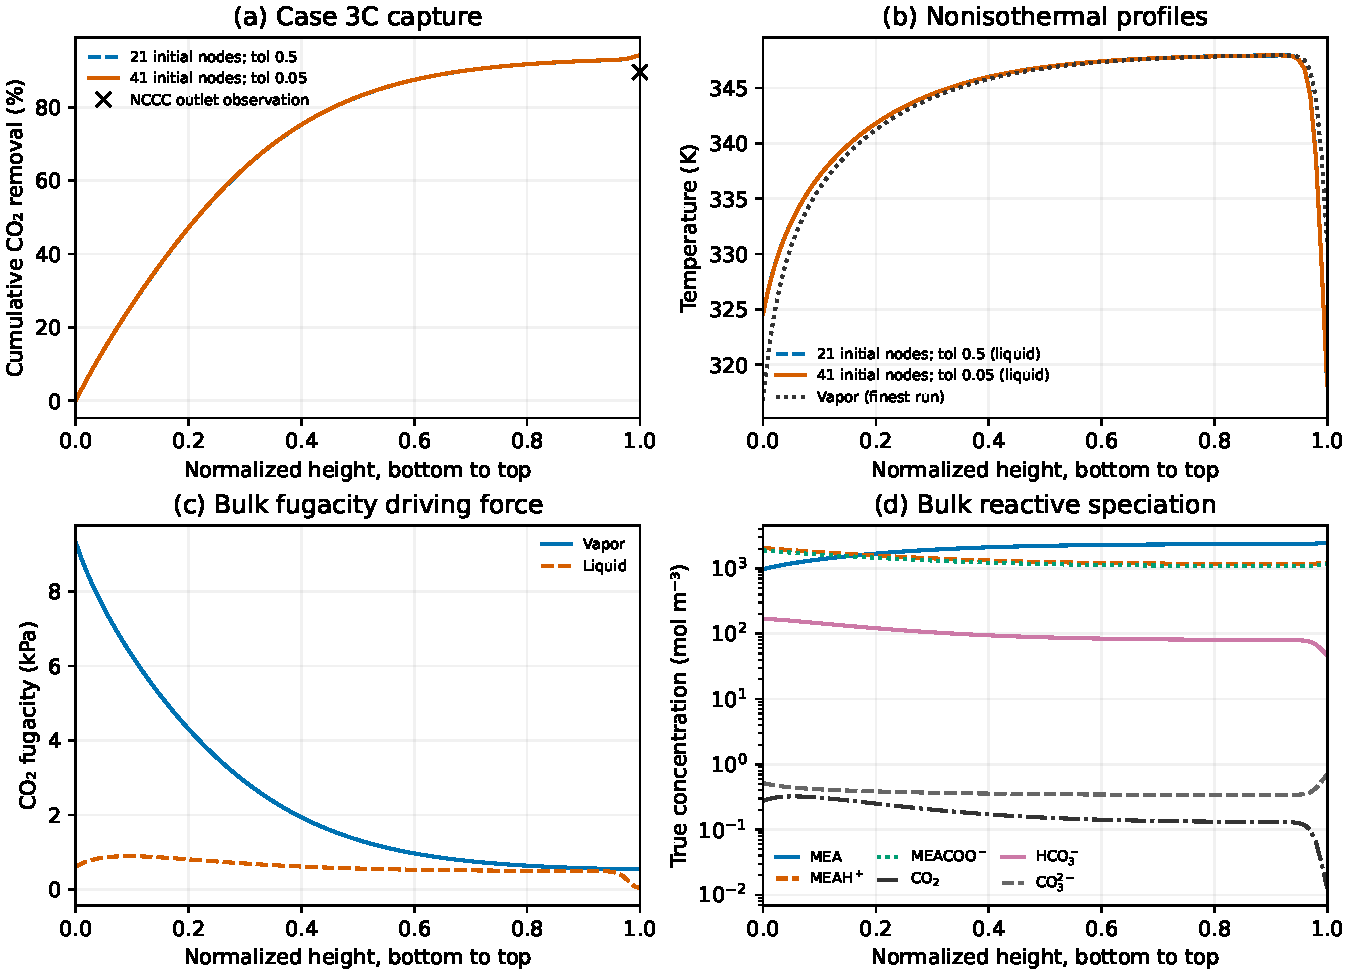
\includegraphics[width=0.98\textwidth]{figures/reactive-case3c-profiles.pdf}
\caption{Coupled nine-species Case 3C profiles with conventional reaction enhancement. The 21- and 41-point initial meshes use collocation tolerances of 0.5 and 0.05. The cross in panel (a) is reported outlet capture (Morgan et al.\ \cite{Morgan2020}); curves are calculated profiles. Panels (c) and (d) use the refined calculation, and panel (d) shows six principal species from the nine-species equilibrium solution. Capture is in percent, temperature in kelvin, fugacity in kilopascals and concentration in \unit{mol.m^{-3}}. Normalized position runs from vapor inlet at 0 to liquid inlet at 1.}
\label{fig:reactive-case3c-profiles}
\end{figure}


\subsubsection*{Numerical verification and computational cost}
% R2: observed refinement
The joint mesh/tolerance refinement changes Case 3C capture by \num{0.005} percentage points and peak liquid temperature by \qty{0.045}{K} (\cref{tab:reactive-numerical-verification}).
Both calculations take two mesh iterations and add one node; the maximum normalized RMS residual decreases from \num{0.125340} to \num{0.043138}, with zero maximum scaled boundary residual.
All nine species remain positive, and net \COtwo{} and water flows vary by less than \qty{3e-14}{mol.s^{-1}} over the exported positions.
At 10,001 sampled positions, the finest additional Case 3C refinement (81 to 121 nodes, tolerance \num{5e-5}) gives an axial net-enthalpy-flow range of \qty{0.134}{W}; its capture differs from the paired refined calculation by less than \num{0.0001} percentage points (\cref{tab:run-diagnostics}).

\begin{table}[pos=htbp]
  \centering
  \caption{Observed joint mesh/tolerance refinement response for the coupled nine-species Case 3C calculation. Both calculations use the same equations and parameters. The iteration rows show the printed maximum normalized RMS residual after each mesh iteration; final residuals below retain additional precision.}
  \label{tab:reactive-numerical-verification}
  \small
  \renewcommand{\arraystretch}{1.12}
  \begin{tabularx}{\textwidth}{@{}Xrr@{}}
    \toprule
    Quantity & Coarser calculation & Refined calculation \\
    \midrule
    Initial / final mesh nodes & 21 / 22 & 41 / 42 \\
    Collocation tolerance & 0.5 & 0.05 \\
    Mesh iterations & 2 & 2 \\
    Maximum RMS residual, iterations 1 $\to$ 2 & $1.64\to0.123$ & $0.0507\to0.0393$ \\
    Final maximum RMS residual & 0.122785 & 0.039322 \\
    Maximum scaled boundary residual & 0 & 0 \\
    Column RHS evaluation batches & 27 & 17 \\
    Jacobian evaluation batches & 6 & 4 \\
    State Jacobian evaluations & 125 & 164 \\
    Liquid equilibrium solves, including profile output & 608 & 551 \\
    \COtwo{} capture (\unit{\percent}) & 94.19959 & 94.20397 \\
    Peak liquid temperature (\unit{K}) & 347.9682 & 347.9399 \\
    Net-enthalpy-flow range, 101 positions (\unit{W}) & 286.440 & 267.572 \\
    \bottomrule
  \end{tabularx}
  \par\smallskip
  \begin{minipage}{\textwidth}\footnotesize
    The continuous equations predict zero net-enthalpy-flow range; the nonzero numerical values are diagnostics, with no asserted energy-error threshold. RHS denotes the right-hand side of the column equations. A batch evaluates all nodes or interval midpoints, not a single axial state. Four Jacobian batches correspond to two node/midpoint pairs. Mesh iterations count outer refinement cycles, not inner Newton steps. Both calculations use boundary tolerance \num{0.001} and a 1000-node limit. Peak memory is reported with the timing study.
  \end{minipage}
\end{table}


% R3: separately measured cost
The three coarse Case 3C repeats have a median BVP wall time of \qty{34.66}{s}, spanning \qtyrange{34.41}{34.89}{s}.
The fastest run uses \qty{34.23}{s} process CPU time and \qty{51.45}{s} total wall time, with peak resident memory \num{203.51} MiB, 21 initial and 22 final nodes, and two mesh iterations.

\subsubsection*{Seven-case comparison}
% R4: capture agreement
Capture agreement varies substantially across the seven NCCC cases (\cref{fig:reactive-seven-case-capture}).
The equally weighted mean absolute error is \num{5.85} percentage points, with the largest signed errors of \num{+11.45} points for Case 6C and \num{-11.93} points for Case 7C.
The opposite signs show that the model does not have a uniform capture bias over these conditions.


\begin{figure}[pos=htbp]
\centering
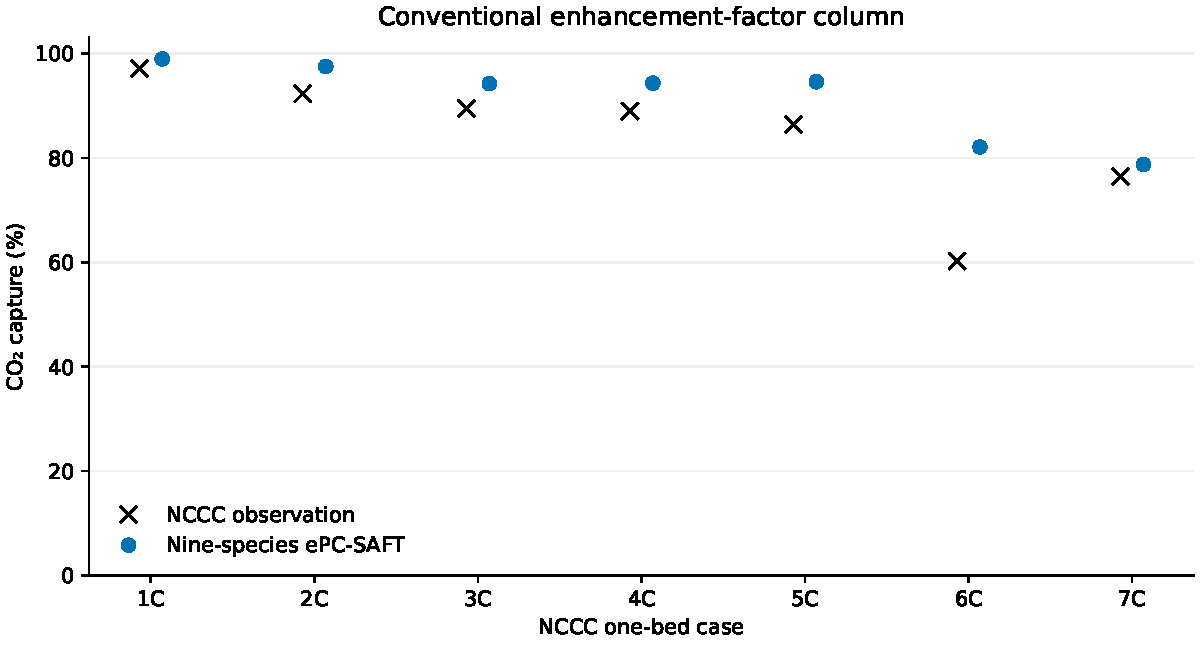
\includegraphics[width=0.9\textwidth]{figures/reactive-seven-case-capture.pdf}
\caption{Predicted and reported capture for NCCC Cases 1C--7C using the coupled nine-species model and observations from Morgan et al.\ \cite{Morgan2020}. Signed errors are prediction minus observation, in percentage points; mean absolute error is \num{5.85} percentage points.}
\label{fig:reactive-seven-case-capture}
\end{figure}


% R5: specific thermal observations
The packing-temperature comparisons expose differences in predicted temperature level and axial shape (\cref{fig:generated-temperature-profiles}).
For Case 3C, both phase curves approach the upper-bed taps near $\zeta=0.6$ and 0.8, but lie above the tap near $\zeta=0.2$; its coarse calculation has \qty{91.54}{\percent} capture and peak liquid temperature \qty{347.91}{K}.
Case 4C overpredicts the three upper taps, while Case 7C predicts a broad elevated-temperature region that is absent from the reported profile, particularly near $\zeta=0.8$.


\begin{figure}[pos=htbp]
\centering
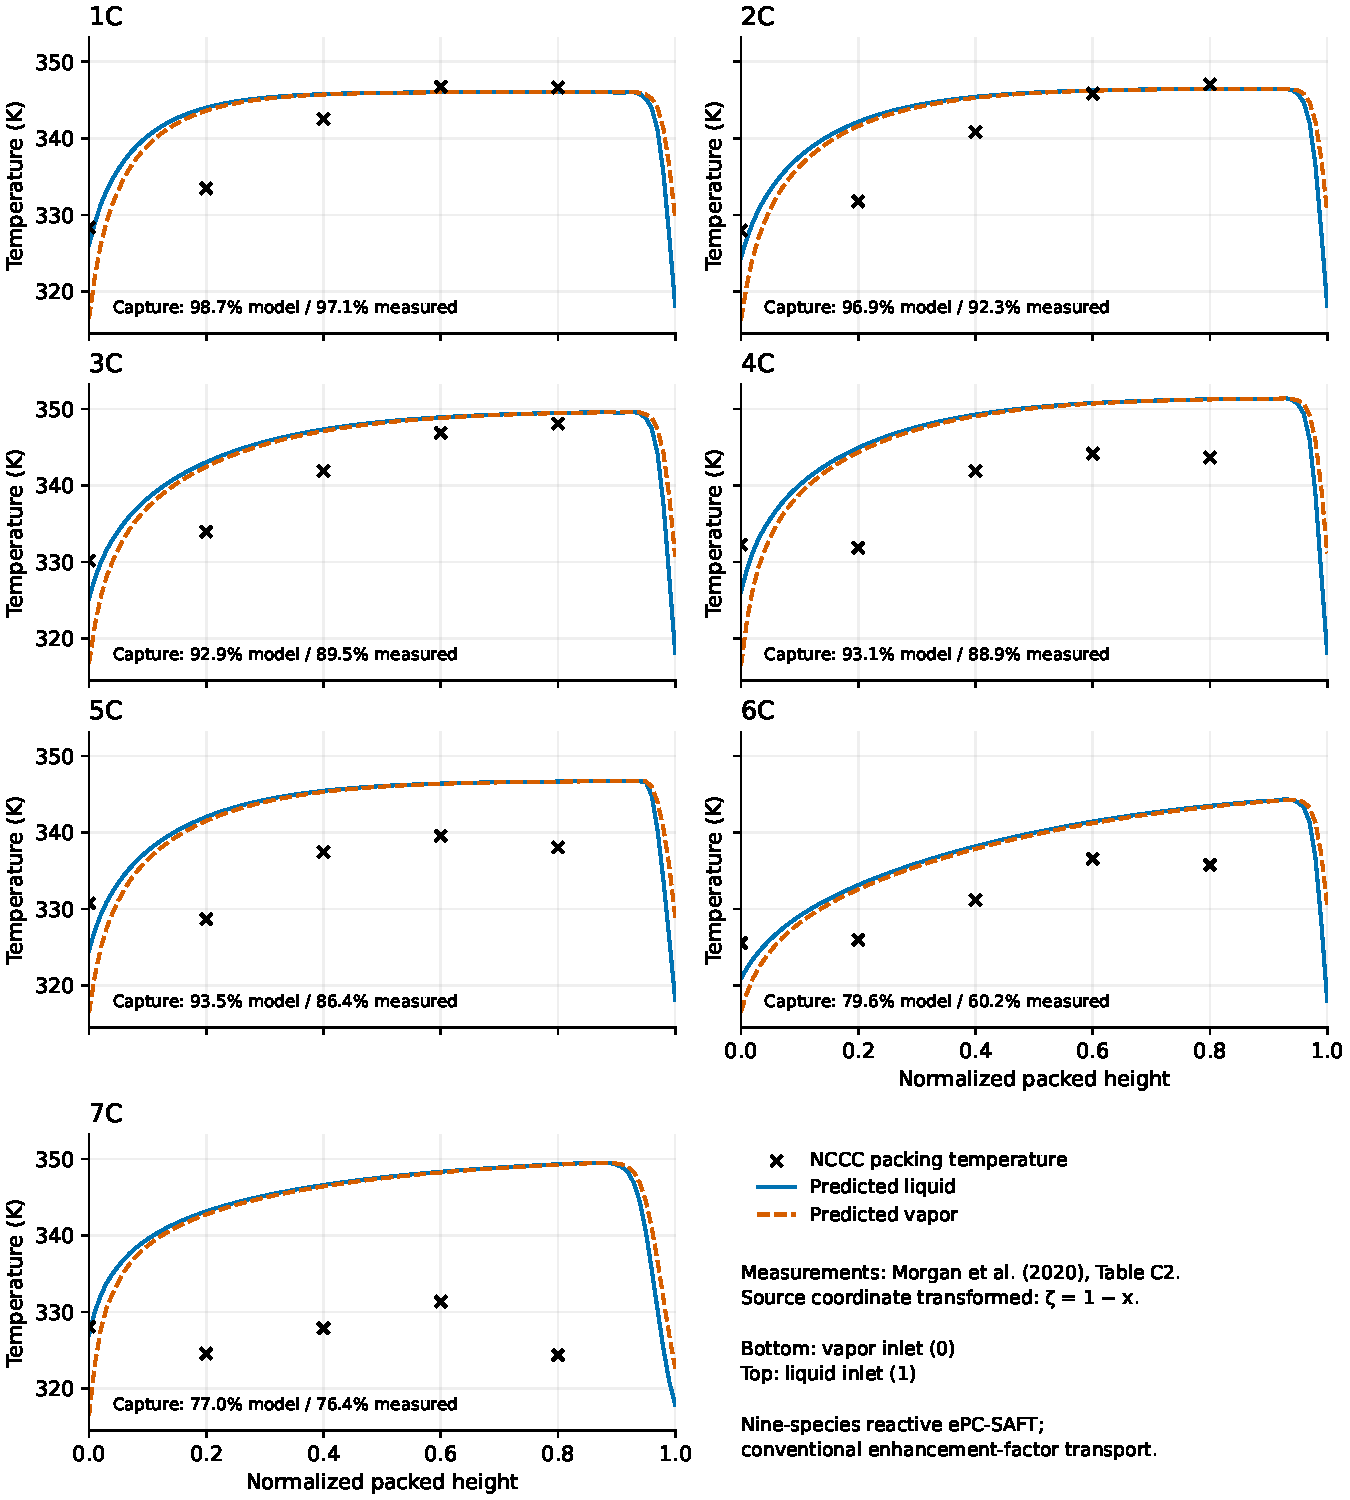
\includegraphics[width=0.98\textwidth]{figures/reactive-seven-case-temperatures.pdf}
\caption{Temperature profiles for the seven one-bed NCCC 2017 C cases. Solid and dashed curves denote liquid and vapor temperatures calculated with coupled nine-species reactive ePC-SAFT and conventional reaction enhancement. Crosses are reported packing temperatures from Table C2 of Morgan et al.\ \cite{Morgan2020}, converted to kelvin and normalized bottom-to-top height $\zeta=1-x$, where $x$ is the source coordinate. The vapor inlet is at zero and liquid inlet at one. The source does not specify a phase-specific sensor designation. Cases 1C--3C use the \qty{318.15}{K} lean-inlet assumption in \cref{tab:nccc-one-bed-scope}.}
\label{fig:generated-temperature-profiles}
\end{figure}


% R6: campaign numerical scope
All seven calculations converge at the campaign settings (\cref{tab:run-diagnostics}), while physical agreement remains uneven. Only Case 3C has the paired refinement, which provides a comparison magnitude for the perturbation responses that follow.
\FloatBarrier

\subsection{Thermodynamic and transport sensitivity}
% R7: thermodynamic capture response
Among the tested equal relative thermodynamic changes, the MEA--water interaction produces the largest capture response (\cref{fig:reactive-parameter-sensitivity}).
Its 0.95 and 1.05 multipliers change capture by \num{-0.82} and \num{+0.76} percentage points from the refined \qty{91.55}{\percent} baseline.
The remaining response magnitudes decrease in the order R5, R4 and \COtwo--water: their paired capture changes are \num{+0.59}/\num{-0.60}, \num{+0.42}/\num{-0.42} and \num{+0.16}/\num{-0.17} points.
Every capture change exceeds the \num{0.005}-point reference refinement difference, but the perturbed range of \qtyrange{90.73}{92.31}{\percent} still exceeds the observed \qty{89.50}{\percent}.


\begin{figure}[pos=htbp]
\centering
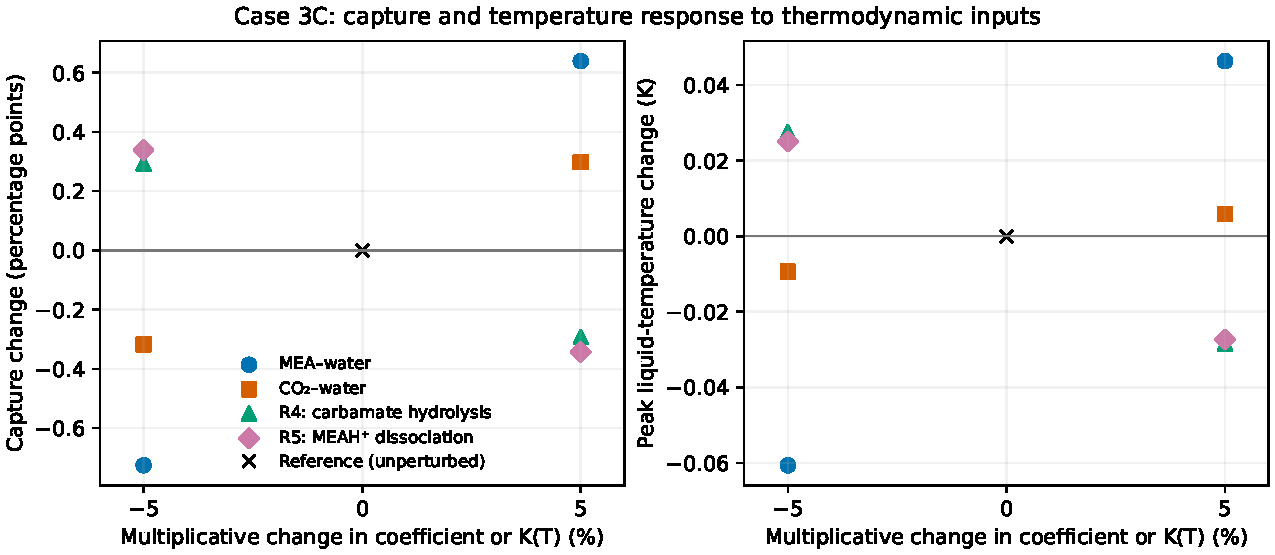
\includegraphics[width=0.98\textwidth]{figures/reactive-parameter-sensitivity.pdf}
\caption{Thermodynamic sensitivity of the coupled nine-species Case 3C model. Points represent separate calculations with one binary interaction coefficient or equilibrium constant multiplied by 0.95 or 1.05; crosses denote the unperturbed reference. R4 denotes carbamate hydrolysis and R5 protonated-MEA dissociation. The reference uses 41 initial nodes and tolerance 0.05, with capture \qty{91.54839}{\percent} and peak liquid temperature \qty{347.86155}{K}. Capture changes are in percentage points and peak liquid-temperature changes are in kelvin.}
\label{fig:reactive-parameter-sensitivity}
\end{figure}


% R8: thermodynamic temperature response
The corresponding peak-temperature changes are small and only partly exceed the \qty{0.045}{K} refinement difference.
MEA--water gives \qty{-0.11}{K} and \qty{+0.10}{K}.
The corresponding R4 changes are \qty{+0.06}{K} and \qty{-0.06}{K}, R5 changes are \qty{+0.06}{K} and \qty{-0.07}{K}, and \COtwo--water changes are \qty{+0.016}{K} and \qty{-0.017}{K}.
The reaction-constant effects modestly exceed it, while the \COtwo--water effects fall below it.

% R9: transport capture response
The liquid-side transfer coefficient has the largest capture effect among the three tested transport inputs (\cref{fig:transport-sensitivity}).
Multipliers of 0.9 and 1.1 give capture changes of \num{-0.53}/\num{+0.40} percentage points, compared with \num{+0.28}/\num{-0.29} for viscosity and \num{+0.08}/\num{-0.09} for free molecular \COtwo{} diffusivity.
The factor-one control reproduces the reference.
All six responses exceed the reference capture refinement difference.


\begin{figure}[pos=htbp]
\centering
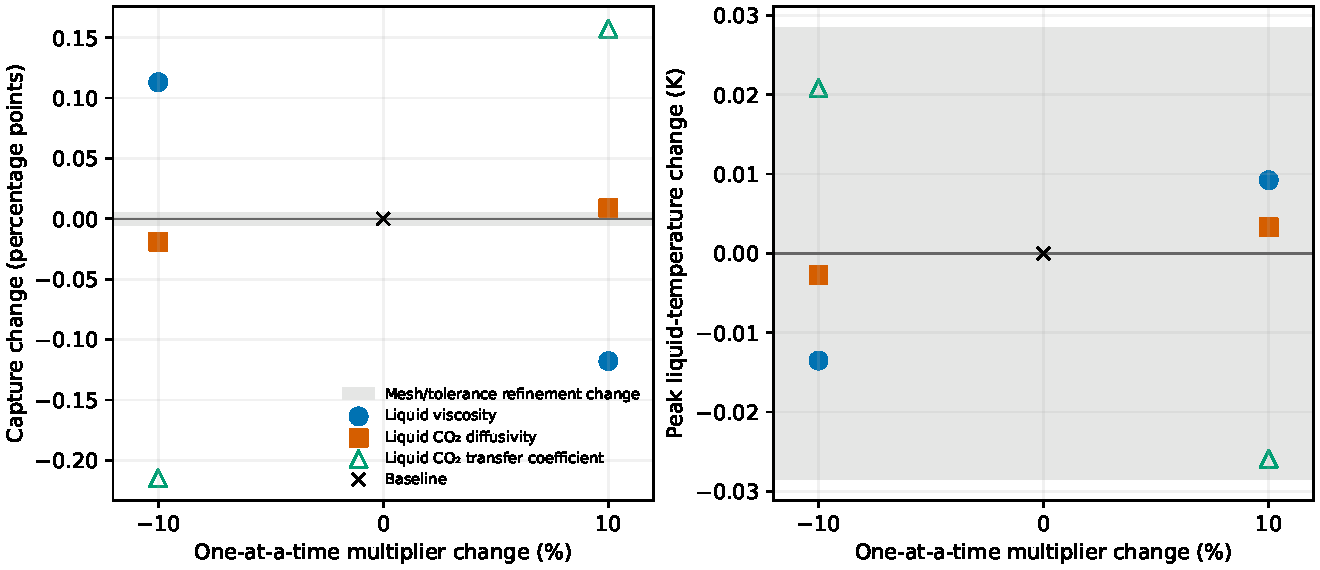
\includegraphics[width=0.98\textwidth]{figures/transport-sensitivity.pdf}
\caption{Transport sensitivity of the coupled nine-species Case 3C model. Points denote separate calculations with liquid viscosity, free liquid \COtwo{} diffusivity or the liquid-side \COtwo{} transfer coefficient multiplied by 0.9 or 1.1, including recalculation of dependent transport and enhancement quantities. The cross denotes the refined reference, with capture \qty{91.54839}{\percent}; capture changes are in percentage points and peak liquid-temperature changes in kelvin. Shading shows the magnitude of the joint mesh/tolerance refinement change.}
\label{fig:transport-sensitivity}
\end{figure}


% R10: coupled transport interpretation
The negative capture response to increased molecular \COtwo{} diffusivity is consistent with the recalculated enhancement and transfer resistances.
For the 1.1 multiplier, median perturbed/reference ratios at matched axial positions are \num{1.047} for $k_L$, \num{0.931} for enhancement and \num{0.975} for their product.
These ratios compare separately solved profiles at matched axial positions.
All peak-temperature changes are below \qty{0.037}{K}, smaller than the \qty{0.045}{K} refinement difference; their signs and ordering are not resolved by that comparison.

% R10b: actual applicability
The baseline calculation extends beyond the documented source ranges of two adopted transport descriptions (\cref{tab:transport-applicability}).
Its Hatta numbers of approximately 320--698 exceed the enhancement source comparison range of 35--165 throughout the profile.
Its peak temperature of \qty{347.86}{K} also exceeds the MEA diffusivity source's \qty{333}{K} upper temperature; the other diffusivity correlations have no documented upper temperature limit.
\FloatBarrier

\subsection{Operating response}\label{sec:operating-response}
% R11: discrete operating results
Six of the seven operating conditions converged, including the coarse baseline with \qty{91.54}{\percent} capture (\cref{fig:operating-response}).
Increasing liquid flow by ten percent at fixed reported dry-gas flow raises capture by \num{0.31} percentage points.
Lean loadings 0.225 and 0.275 mol \COtwo{} per mol MEA give changes of \num{+3.75} and \num{-6.86} points relative to 0.25, while liquid-inlet temperatures \qty{313.15}{K} and \qty{323.15}{K} give \num{+0.11} and \num{-0.08} points relative to \qty{318.15}{K}.


\begin{figure}[pos=htbp]
\centering
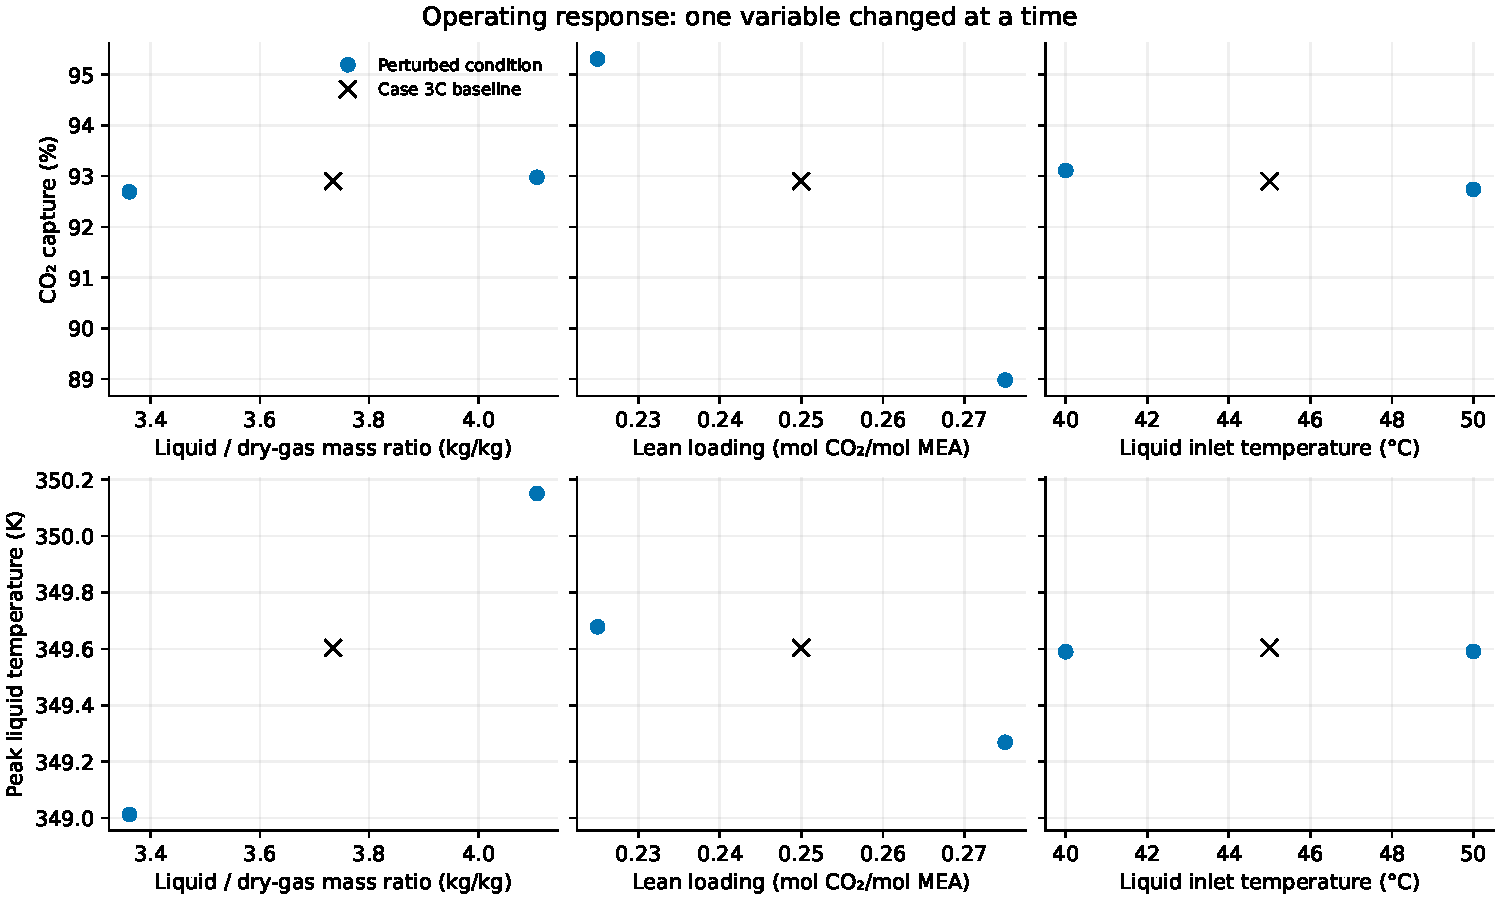
\includegraphics[width=0.98\textwidth]{figures/reactive-operating-response.pdf}
\caption{Operating response of the coupled nine-species Case 3C model. Circles denote discrete one-at-a-time predictions; crosses denote the unperturbed baseline. The baseline has $L/G=3.73423$ (liquid mass/reported dry gas mass), loading 0.25 mol \COtwo{} per mol MEA and liquid-inlet temperature \qty{318.15}{K}. Capture is in percent and peak liquid temperature in kelvin. Liquid mass flow changes at fixed reported dry-gas flow for the mass-ratio comparison. The lower liquid-to-gas condition did not converge and is omitted.}
\label{fig:operating-response}
\end{figure}


% R12: joint capture and temperature interpretation
Lower lean loading increases available solvent capacity and gives the largest positive capture response among these specified changes.
Lower loading raises free MEA and lowers the liquid \COtwo{} fugacity; near the gas inlet, this increases the modeled driving force.
Peak liquid-temperature changes are \qty{+0.61}{K} for higher liquid flow and \qty{+0.25}{K}/\qty{-0.83}{K} for the two loading changes.
The colder and warmer liquid inlets give peak changes of \qty{+0.02}{K} and \qty{-0.01}{K}, both below the refinement difference.

\FloatBarrier

\subsection{Interpretation and future work}
% R14: integrated interpretation
The calculations connect reactive bulk thermodynamics to column response, while physical disagreement persists despite small capture changes under the tested refinement.
The refined Case 3C capture error of \num{2.05} percentage points is much larger than its \num{0.005}-point refinement change, and Cases 6C and 7C have still larger physical discrepancies.
The reduced vapor-EOS composition and the extrapolated enhancement and transport correlations limit interpretation; their individual contributions to the error are not resolved.
The lean-inlet temperature assumed for Cases 1C--3C is a bounded input uncertainty: in Case 3C, liquid-inlet temperatures of \qty{313.15}{K} and \qty{323.15}{K} change capture by \num{+0.11} and \num{-0.08} percentage points relative to \qty{318.15}{K} (\cref{sec:operating-response}), small against the \num{2.05}-point refined capture error.

% R15: limitations and next steps
The film, parameter and optimization questions raised by these results were examined with a twelve-state conserved formulation of the same absorber, discretized in conservative upwind cells and solved with IPOPT \cite{Wachter2006}.
This formulation differs from the nine-species model reported above, so its capture errors are not directly comparable with the \num{5.85}-point mean absolute error of that model.
A finite-rate reactive film computes \COtwo{} transfer from ePC-SAFT bulk and interfacial speciation, with an \NtwoO{}-analogy Henry constant and no empirical enhancement factor.
Across Cases 2C--7C at 129 axial nodes, its capture mean absolute error is \num{5.45} percentage points, against \num{6.05} for an equilibrium-manifold film and \num{6.28} for the enhancement factor; this order holds at 17, 33, 65 and 129 nodes, and Case 1C is omitted because the enhancement-factor calculation did not converge on the two finest meshes.
Mesh refinement raises the error of all three films, and at 129 nodes all three underpredict Case 7C capture by \num{8.8} to \num{17.4} percentage points, with changes of \num{1.6} to \num{1.8} points still occurring between 65 and 129 nodes, so Case 7C is not resolved with respect to the axial mesh.
With the jointly fitted MEA parameter set, which also changes the reaction and caloric inputs, the seven-case capture mean absolute error at 33 nodes is \num{4.58} percentage points, against \num{4.79} with the earlier set; without Case 7C, the earlier set is better at \num{4.27} against \num{4.87} points, so the joint fit does not consistently improve the absorber prediction.
Constrained optimization with exact first derivatives was verified for the minimum solvent flow that gives \qty{90}{\percent} capture in Case 3C with the equilibrium-manifold film.\footnote{These optimization calculations used the MA57 linear solver from HSL, a collection of Fortran codes for large-scale scientific computation, \url{https://www.hsl.rl.ac.uk/}.}
The calculated optimum lies \qty{2.47}{\percent}, \qty{5.95}{\percent} and \qty{9.25}{\percent} above the reference solvent flow at 17, 33 and 65 nodes, so the mesh-independent solvent requirement remains unresolved.
All of these capture results are comparisons between model and measurement, not validation.

% R16: remaining outlook
A matched ePC-SAFT versus eNRTL comparison in this column model, with fixed configuration, inlet conditions and transport assumptions and internally consistent parameterizations \cite{Akula2023a,Zhang2011}, would quantify the calibration data and effort each model requires.
Tests with diethanolamine (DEA), methyldiethanolamine (MDEA), 2-amino-2-methyl-1-propanol (AMP), piperazine (PZ) and blends would show which component, association and ionic inputs transfer and which require solvent-specific calibration.


    \section{Conclusions}
% C1: coupled formulation and physical evaluation
The coupled formulations connect five-reaction, nine-species liquid equilibrium and ePC-SAFT bulk-phase properties to nonisothermal MEA absorber balances.
ePC-SAFT supplies the density, enthalpies, heat capacities, phase and reaction equilibrium, \COtwo{} solubility and water fugacities these balances use, while surface tension, transport, kinetics and packing performance remain correlations.
No thermodynamic parameter is fitted to the seven NCCC one-bed cases, so the capture and temperature comparisons are predictions.

% C2: twelve-state film comparison
In the twelve-state conserved formulation, a finite-rate reactive film with the ePC-SAFT Henry coefficient predicts capture with a mean absolute error of \num{3.55} percentage points at 129 axial nodes, against \num{4.52} for an equilibrium-manifold film and \num{7.51} for conventional enhancement.
The \NtwoO{}-analogy solubility gives \num{3.61} points, so these cases do not distinguish the two solubility bases.
Every film overpredicts Case 6C, Case 7C capture is not resolved with respect to the axial mesh, and the calculated liquid temperatures exceed the Case 7C packing temperatures by up to \qty{24}{K}.

% C3: nine-species numerical behavior and property sources
The nine-species BVP formulation with conventional enhancement overpredicts all seven cases, with a mean absolute error of \num{5.86} percentage points.
Its refined Case 3C calculation predicts \qty{92.91}{\percent} capture against \qty{89.50}{\percent} observed; mesh refinement changes capture by \num{0.005} points, and one coarse solution requires about \qty{17}{s} of BVP wall time.
Replacing empirical density and calorics with ePC-SAFT lowers capture in every case and raises the packing-temperature error; in Case 3C the capture change comes mostly from the lower ePC-SAFT water vaporization enthalpy.

% C4: thermodynamic, transport and operating insights
The MEA--water interaction produces the largest capture response among the tested thermodynamic inputs and the liquid-side transfer coefficient the largest among the transport inputs, but neither closes the Case 3C capture gap within the tested ranges.
Lean loadings of 0.225 and 0.275 mol \COtwo{} per mol MEA change capture by \num{+2.41} and \num{-3.92} points relative to 0.25, identifying solvent loading as the most influential operating variable under the tested conditions.

The temperature comparison is qualitative because the source does not identify the measured phase; the conventional enhancement and the transport correlations used beyond their source ranges constrain predictive interpretation.

% C5: contribution and forward program
The formulations give a direct connection from component-level molecular and ionic descriptions to column-scale observables and operating response.
The minimum Case 3C solvent flow for \qty{90}{\percent} capture from the twelve-state model moves toward the reference flow with mesh refinement, leaving its mesh-independent value unresolved.
A direct ePC-SAFT/eNRTL comparison and tests with other amines would evaluate how thermodynamic parameter reuse contributes to solvent selection and absorber design.

\clearpage
\nolinenumbers
\raggedbottom


    \appendix
    \crefalias{section}{appendix}

    \section{Property and transport correlations}\label{sec:properties}
% A1: apparent property basis
In the reported calculations ePC-SAFT supplies the liquid and vapor densities, enthalpies and heat capacities (\cref{sec:model-framework}).
The density, heat-capacity and enthalpy correlations below serve only as the comparison property source of \cref{sec:nine-species-results}; the surface-tension, conductivity, viscosity and diffusivity correlations enter every calculation.
The auxiliary property correlations use apparent liquid components \COtwo, MEA and water and the full wet-gas composition \COtwo, water, nitrogen and oxygen.
These bases differ from the nine true liquid species and the reduced neutral vapor EOS composition.
Apparent liquid mass fractions are \(w_i=x_i\mathrm{MW}_i/\sum_jx_j\mathrm{MW}_j\), where \(x_i\) are apparent mole fractions and \(\mathrm{MW}_i\) are component molar masses.
The property routines use liquid molar masses (0.04401, 0.06108, 0.01802) and vapor molar masses (0.04401, 0.01802, 0.02801, 0.032) in \unit{kg.mol^{-1}}; the separately specified EOS values are listed in \cref{tab:epcsaft-pure-parameters}.
\subsection{Physical carbon dioxide solubility}
% A2: physical solubility
The physical solubility correlation follows the \NtwoO{} analogy \cite{Jiru2012}.
It generates the starting profile of the nine-species model and supplies the interfacial solubility of the twelve-state finite-rate film in its \NtwoO{}-analogy variant (\cref{subsec:twelve-state}).
Here $\overline w_i=w_i/(w_{\MEA}+w_{\HtwoO})$ is a CO$_2$-free solvent mass fraction, and the resulting concentration-based Henry coefficient differs from the ePC-SAFT Henry coefficient $H_{\mathrm{bulk}}$ of \cref{subsec:transport}.
\begin{align}
H_{\NtwoO,\MEA} &= \left(A_{\NtwoO,\MEA} \times 10^5\right) e^{\frac{-B_{\NtwoO,\MEA}}{T^{\liq}}} && \left(\unit{Pa\,m^3\,mol^{-1}}\right)\\
H_{\NtwoO,\HtwoO} &= \left(A_{\NtwoO,\HtwoO} \times 10^6\right) e^{\frac{-B_{\NtwoO,\HtwoO}}{T^{\liq}}} && \left(\unit{Pa\,m^3\,mol^{-1}}\right)\\
H_{\COtwo,\MEA} &= H_{\NtwoO,\MEA} \frac{H_{\COtwo, \HtwoO}}{H_{\NtwoO,\HtwoO}} && \left(\unit{Pa\,m^3\,mol^{-1}}\right)
\end{align}
The corresponding expression for $\COtwo$ solubility in $\HtwoO$ is
\begin{align}
H_{\COtwo, \HtwoO} &= \left(A_{\COtwo, \HtwoO} \times 10^6\right) e^{\frac{-B_{\COtwo, \HtwoO}}{T^{\liq}}} && \left(\unit{Pa\,m^3\,mol^{-1}}\right)
\end{align}
A deviation term $R_a$ with fitted coefficients $a_1$, $a_2$, $a_3$ and $b$ accounts for nonideal mixed-solvent solubility.
\begin{align}
R_{a} &= \left(a_1+a_2 \left(T^{\liq}-273.15\right)+a_3 \left(T^{\liq}-273.15\right)^2+b \overline w_{\HtwoO}\right) \overline w_{\MEA} \overline w_{\HtwoO}
&& \text{dimensionless}\\
\Lambda_H &= \overline w_{\MEA} \ln\left(H_{\COtwo,\MEA}/H^\circ\right)+\overline w_{\HtwoO} \ln\left(H_{\COtwo,\HtwoO}/H^\circ\right)
&& \text{dimensionless}\\
H_{\COtwo,\text{mix}} &= H^\circ e^{R_{a} + \Lambda_H} && \left(\unit{Pa\,m^3\,mol^{-1}}\right)
\end{align}


The logarithms use $H^\circ=\qty{1}{Pa.m^3.mol^{-1}}$ and temperature numerically in kelvin.
The coefficient pairs $(A,B)$ are $(2.448,1348)$ for N$_2$O--MEA, $(8.449,2283)$ for N$_2$O--water and $(3.52,2113)$ for CO$_2$--water, with $B$ in kelvin and the pressure-volume prefactors shown above.
The adopted mixture coefficients are
\begin{equation}
(a_1,a_2,a_3,b)=(1.70981,0.03972,-4.3\times10^{-4},-2.20377),
\end{equation}
with $a_1$ and $b$ dimensionless, $a_2$ in \unit{K^{-1}} and $a_3$ in \unit{K^{-2}}.

\subsection{Density and surface tension}
% A3: density and surface tension
The phase-mean molar masses are \(\mathrm{MW}_T^\liq=\sum_i x_i\mathrm{MW}_i\) and \(\mathrm{MW}_T^\vap=\sum_i y_i\mathrm{MW}_i\), using apparent phase compositions.
The comparison density correlations are taken from Morgan et al. \cite{Morgan2015}, with an ideal-gas vapor density.
Apparent liquid mole fractions are used.
Component-volume correlations return \unit{mL\,mol^{-1}} before the factor $10^{-6}$ converts them to \unit{m^3\,mol^{-1}}; temperatures are in kelvin and molar masses in \unit{kg\,mol^{-1}}.
\begin{align}
\shortintertext{\quad\; Liquid Density}
V^{\liq}_{\COtwo} &=  10^{-6}\left[a_{\COtwo}+(b_{\COtwo}+c_{\COtwo}x_{\MEA})x_{\MEA}\right]
&& \left(\unit{m^{3}\,mol^{-1}}\right)\\
V^{\liq}_{\MEA} &=  10^{-6}\left[\frac{1000\,\text{MW}_{\MEA}}{a_{\MEA} (T^{\liq})^2 + b_{\MEA} T^{\liq} + c_{\MEA}} + x_{\HtwoO}(d_{\MEA}+e_{\MEA}x_{\MEA})\right]
&& \left(\unit{m^{3}\,mol^{-1}}\right)\\
V^{\liq}_{\HtwoO} &=  10^{-6}\frac{1000\,\text{MW}_{\HtwoO}}{a_{\HtwoO} (T^{\liq})^2 + b_{\HtwoO} T^{\liq} + c_{\HtwoO}}
&& \left(\unit{m^{3}\,mol^{-1}}\right)\\
V^{\liq} &= V^{\liq}_{\COtwo}x_{\COtwo} + V^{\liq}_{\MEA}x_{\MEA} + V^{\liq}_{\HtwoO}x_{\HtwoO}
&& \left(\unit{m^{3}\,mol^{-1}}\right)\\
\rho ^{\liq}_{mol} &= \frac{1}{V^{\liq}}
&& \left(\unit{mol\,m^{-3}}\right)\\
\rho ^{\liq}_{mass} &= \rho ^{\liq}_{mol}\text{MW}^{\liq}_{T}
&& \left(\unit{kg\,m^{-3}}\right)\\
\shortintertext{\quad\; Vapor Density}
\rho ^{\vap}_{mol} &= \frac{P}{RT^{\vap}}
&& \left(\unit{mol\,m^{-3}}\right)\\
\rho ^{\vap}_{mass} &= \rho ^{\vap}_{mol}\text{MW}^{\vap}_{T}
&& \left(\unit{kg\,m^{-3}}\right)
\end{align}
For the 53 loaded-solution densities of Amundsen et al.\ \cite{Amundsen2009} that are outside the parameter-fit objective, the ePC-SAFT liquid density has a mean absolute deviation of \qty{0.51}{\percent}, against \qty{3.49}{\percent} for this correlation, which lies below every one of these points.
For the 30 unloaded densities outside the fit objective the deviations are \qty{0.20}{\percent} and \qty{0.46}{\percent}.


The surface-tension correlation is taken from Morgan et al. \cite{Morgan2015}.
Here $r=w_{\MEA}/(w_{\MEA}+w_{\HtwoO})$ is the solvent-basis MEA mass fraction, and $\alpha=x_{\COtwo}/x_{\MEA}$ uses apparent liquid mole fractions.
\begin{align}
\shortintertext{\quad\; Component and composition-dependent contributions}
\sigma _{\COtwo} &= S_1 r^2+S_2 r+S_3+T^{\liq} \left(S_4 r^2+S_5 r+S_6\right)
&& \left(\unit{N\,m^{-1}}\right)\\
\sigma _{\MEA} &= c_{1,\MEA} \left(1-\frac{T^{\liq}}{T_{c,\MEA}}\right)^{c_{2,\MEA}+c_{3,\MEA} \frac{T^{\liq}}{T_{c,\MEA}}+c_{4,\MEA} \left(\frac{T^{\liq}}{T_{c,\MEA}}\right)^2}
&& \left(\unit{N\,m^{-1}}\right)\\
\sigma _{\HtwoO} &= c_{1,\HtwoO} \left(1-\frac{T^{\liq}}{T_{c,\HtwoO}}\right)^{c_{2,\HtwoO}+c_{3,\HtwoO} \frac{T^{\liq}}{T_{c,\HtwoO}}+c_{4,\HtwoO} \left(\frac{T^{\liq}}{T_{c,\HtwoO}}\right)^2}
&& \left(\unit{N\,m^{-1}}\right)\\
\shortintertext{\quad\; Additional terms provide continuous values over the fitted range of $r$}
A &= a+b \alpha+c {\alpha}^2+d r+e r^2
&& \text{dimensionless}\\
B &= f+g \alpha+h {\alpha}^2+i r+j r^2
&& \text{dimensionless}\\
\shortintertext{\quad\; The final expression}
\sigma _{\text{mix}} &= \sigma_{\HtwoO}+\left(\sigma_{\COtwo}-\sigma_{\HtwoO}\right) A x_{\COtwo}+\left(\sigma_{\MEA}-\sigma_{\HtwoO}\right) B x_{\MEA}
&& \left(\unit{N\,m^{-1}}\right)
\end{align}


The density coefficients in the displayed numerical temperature and volume convention are
\begin{align*}
(a,b,c)_{\COtwo}&=(10.2074,207.0,-563.3701),\\
(a,b,c)_{\MEA}&=(-5.35162\times10^{-7},-4.51417\times10^{-4},1.19451),\\
(d,e)_{\MEA}&=(-2.2642,3.0059),\\
(a,b,c)_{\HtwoO}&=(-3.2484\times10^{-6},0.00165,0.793).
\end{align*}
The pure-solvent surface-tension coefficients are
\begin{align*}
(c_1,c_2,c_3,c_4,T_c)_{\MEA}&=(0.09945,1.067,0,0,614.45),\\
(c_1,c_2,c_3,c_4,T_c)_{\HtwoO}&=(0.18548,2.717,-3.554,2.047,647.13),
\end{align*}
with $c_1$ in \unit{N.m^{-1}} and $T_c$ in kelvin.
The adopted composition-dependent coefficients are
\begin{align*}
(S_1,S_2,S_3)&=(-0.00589934906113,0.00175020536429,0.129650182728),\\
(S_4,S_5,S_6)&=(1.26444768126\times10^{-5},-5.73954817200\times10^{-6},-1.89690055342\times10^{-4}),\\
(a,b,c,d,e)&=(1070.65668318,-2578.78134209,3399.24113311,-2352.47410135,2960.24753688),\\
(f,g,h,i,j)&=(3.06684894924,-1.79435372760,-7.21242190758,2.97502322397,-10.5738529302).
\end{align*}
$S_1$--$S_3$ have units \unit{N.m^{-1}}, $S_4$--$S_6$ have units \unit{N.m^{-1}.K^{-1}}, and the remaining coefficients are dimensionless.
The CO$_2$ contribution depends on solvent composition and is not a pure-component surface tension.

\subsection{Heat capacity and enthalpy}
% A4: empirical calorics
The heat-capacity and enthalpy correlations of this subsection are the comparison caloric source.
The solvent heat-capacity method follows Hilliard \cite{Hilliard2008}.
The polynomial argument is Celsius temperature $T_C=T^{\liq}-273.15$, with $T^{\liq}$ in kelvin and molar masses in \unit{kg\,mol^{-1}}.
\begin{align}
C^{\liq}_{p,\MEA} &= 1000 \times \text{MW}_{\MEA} \sum_{i=0}^{4} c_{i,\MEA}(T^{\liq}-273.15)^i
&& \left(\unit{J\,mol^{-1}\,K^{-1}}\right)\\
C^{\liq}_{p,\HtwoO} &= 1000 \times \text{MW}_{\HtwoO} \sum_{i=0}^{4} c_{i,\HtwoO}(T^{\liq}-273.15)^i
&& \left(\unit{J\,mol^{-1}\,K^{-1}}\right)\\
C^{\liq}_{p,\COtwo} &= \frac{x_{\MEA} C^{\liq}_{p,\MEA} + x_{\HtwoO} C^{\liq}_{p,\HtwoO}}{x_{\COtwo}} \left( \frac{1}{1 - w_{\COtwo}} - 1\right)
&& \left(\unit{J\,mol^{-1}\,K^{-1}}\right)
\end{align}


The adopted solvent coefficient vectors $(c_0,\ldots,c_4)$ are $(2.6161,0.003706,3.787\times10^{-6},0,0)$ for MEA and $(4.2107,-0.001696,2.568\times10^{-5},-1.095\times10^{-7},3.038\times10^{-10})$ for water, giving mass heat capacity numerically in \unit{kJ.kg^{-1}.K^{-1}} before molar conversion.
The additive enthalpy model uses these solvent correlations adapted from Akula \cite{Akula2023}, constant reference offsets, and a fixed \COtwo{} absorption enthalpy.
It is separate from the EOS activity calculation; $T_{ref}=\qty{298.15}{K}$.
The derivative below follows this correlation, including composition weights.
\begin{align}
\shortintertext{\quad\; Apparent-component enthalpies}
H^{\liq}_{\COtwo} &= -84000
&& \left(\unit{J\,mol^{-1}}\right)\\
H^{\liq}_{\MEA} &= \int_{T_{ref}}^{T^{\liq}} C_{p,\MEA} \,\differential T^{\liq} - 58000
&& \left(\unit{J\,mol^{-1}}\right)\\
H^{\liq}_{\HtwoO} &= \int_{T_{ref}}^{T^{\liq}} C_{p,\HtwoO} \,\differential T^{\liq} - 49990
&& \left(\unit{J\,mol^{-1}}\right)\\
\shortintertext{\quad\; Total enthalpy for liquid phase}
H^{\liq}_{T} &= \sum_{i} x_iH^{\liq}_{i}
&& \left(\unit{J\,mol^{-1}}\right)\\
\shortintertext{\quad\; Temperature derivative at fixed apparent composition}
\left(\pdv{H^{\liq}_{T}}{T^{\liq}}\right)_{\boldsymbol{x}} &= x_{\MEA} C^{\liq}_{p,\MEA} + x_{\HtwoO} C^{\liq}_{p,\HtwoO}
&& \left(\unit{J\,mol^{-1}\,K^{-1}}\right)
\end{align}
With ideal-gas vapor enthalpies, the water offset of \qty{49.99}{kJ.mol^{-1}} sets the water vaporization enthalpy of this correlation at $T_{ref}$, against \qtyrange{42.7}{43.2}{kJ.mol^{-1}} for water transfer from ePC-SAFT at \qty{313.15}{K} and \qty{43.34}{kJ.mol^{-1}} for pure water.
This difference causes most of the capture difference between the two property sources (\cref{sec:nine-species-results}).
The ePC-SAFT calorics under-predict the differential \COtwo{} absorption enthalpies of Kim and Svendsen \cite{Kim2007}: the mean signed deviation is \qty{-2.43}{kJ.mol^{-1}} for 37 points at \qty{313.15}{K} and \qty{-9.30}{kJ.mol^{-1}} for 29 points at \qty{353.15}{K}, with 13 and 2 points within the stated \qty{2.2}{\percent} uncertainty.


Vapor enthalpies use the same ideal-gas heat-capacity coefficients as the vapor heat-capacity model:
\begin{align}
H_i^\vap &= R\biggl[A_i(T^\vap-T_{ref})+\frac{B_i}{2}\bigl((T^\vap)^2-T_{ref}^2\bigr)\notag\\
&\qquad-C_i\left(\frac{1}{T^\vap}-\frac{1}{T_{ref}}\right)\biggr],\\
H_T^\vap&=\sum_i y_iH_i^\vap,\\
C_{p,T}^\vap&=R\sum_i y_i\left(A_i+B_iT^\vap+\frac{C_i}{(T^\vap)^2}\right).
\end{align}
Enthalpies are in \unit{J\,mol^{-1}} and heat capacities in \unit{J\,mol^{-1}\,K^{-1}}.
The coefficient triples \((A_i,B_i,C_i)\), with \(B_i\) in \unit{K^{-1}} and \(C_i\) in \unit{K^2}, are
\begin{align*}
\COtwo &: (5.457,1.045\times10^{-3},-1.157\times10^5),\\
\HtwoO &: (3.47,1.45\times10^{-3},0.121\times10^5),\\
\Ntwo &: (3.28,0.593\times10^{-3},0.04\times10^5),\\
\Otwo &: (3.639,0.506\times10^{-3},-0.227\times10^5).
\end{align*}

\subsection{Thermal conductivity}
% A5: vapor thermal conductivity
The vapor heat-transfer calculation uses the following pure-component correlations and viscosity-based mixing rule.
\begin{align}
k^{t}_{i} = \frac{A_i T^{B_i}}{1 + \frac{C_i}{T} + \frac{D_i}{T^2}}
\qquad \left(\unit{J\,s^{-1}\,m^{-1}\,K^{-1}}\right)
\end{align}

The vapor mixture uses
\begin{equation}
k_t^\vap=\sum_i\frac{y_i k_i^t}{\sum_j y_j\theta_{ij}},
\end{equation}
where \(\theta_{ij}\) is the viscosity-based Wilke factor defined in the vapor-viscosity equations below, not a conductivity ratio.
The pure-component coefficients \((A_i,B_i,C_i,D_i)\), in the displayed SI correlation, are
\begin{align*}
\COtwo &: (3.69,-0.3838,964,1.86\times10^6),\\
\HtwoO &: (6.204\times10^{-6},1.3973,0,0),\\
\Ntwo &: (0.000331,0.7722,16.323,373.72),\\
\Otwo &: (0.00045,0.7456,56.699,0).
\end{align*}


\subsection{Viscosity}
% A6: viscosity
The liquid correlation follows the form of Morgan et al.\ \cite{Morgan2015a}, with the modified coefficient vector stated below and its source applicability distinguished in \cref{tab:transport-applicability}.
\paragraph{Liquid viscosity.}
The water-reference coefficients are $A=\qty{1.002e-3}{Pa\,s}$, $B=1.3272$, $C=\qty{0.001053}{K^{-1}}$ and $D=\qty{168.15}{K}$.
Here \(r=w_{\MEA}/(w_{\MEA}+w_{\HtwoO})\) and $r_\mu=100r$ is the MEA mass percentage on the CO$_2$-free solvent basis, and $\alpha=x_{\COtwo}/x_{\MEA}$ is the apparent loading.
For temperature in kelvin, the correlation coefficients are
\begin{align*}
a=g&=-0.0854041877181552,& b&=2.72913373574306,\\
c&=35.1158892542595,& d&=1805.52759876533,\\
e&=0.00716025669867574,& f&=0.0106488402285381.
\end{align*}
\begin{align}
\mu ^{\liq}_{\HtwoO} &= A \times 10^\frac{B\left(293.15 - T^{\liq} - C\left(T^{\liq} - 293.15\right)^2\right)}{T^{\liq} - D}
&& \left(\unit{Pa\,s}\right)\\
\Delta_\mu &= \frac{r_\mu\left[T^{\liq}(a r_\mu+b)+c r_\mu+d\right]
\left[\alpha(e r_\mu+f T^{\liq}+g)+1\right]}{(T^{\liq})^2}
&& \text{dimensionless}\\
\mu ^{\liq}_{\text{mix}} &= \mu ^{\liq}_{\HtwoO} \exp(\Delta_\mu)
&& \left(\unit{Pa\,s}\right)
\end{align}
\vspace{.5cm}
\paragraph{Vapor viscosity.}
\begin{align}
\mu ^{\vap}_{\COtwo} &= \frac{2.148 \times 10^{-6} \ (T^{\vap})^{0.46}}{1+\frac{290}{T^{\vap}}}
&& \left(\unit{Pa\,s}\right)\\
\mu ^{\vap}_{\HtwoO} &= 1.7096\times 10^{-8} \ (T^{\vap})^{1.1146}
&& \left(\unit{Pa\,s}\right)\\
\mu ^{\vap}_{\Ntwo} &= 1.781\times10^{-5}\frac{300.55+111}{T^{\vap}+111}\left(\frac{T^{\vap}}{300.55}\right)^{3/2}
&& \left(\unit{Pa\,s}\right)\\
\mu ^{\vap}_{\Otwo} &= 2.018\times10^{-5}\frac{292.25+127}{T^{\vap}+127}\left(\frac{T^{\vap}}{292.25}\right)^{3/2}
&& \left(\unit{Pa\,s}\right)\\
\theta_{ij} &= \frac{1 + 2\,\sqrt{\frac{\mu^{\vap}_{i}}{\mu^{\vap}_{j}}}\left(\frac{\text{MW}^{\vap}_{j}}{\text{MW}^{\vap}_{i}}\right)^{0.25} + \frac{\mu^{\vap}_{i}}{\mu^{\vap}_{j}}\left(\frac{\text{MW}^{\vap}_{j}}{\text{MW}^{\vap}_{i}}\right)^{0.5}}{\sqrt{8 + 8\,\frac{\text{MW}^{\vap}_{i}}{\text{MW}^{\vap}_{j}}}}
&& \text{dimensionless}\\
\theta_{ji} &= \frac{\mu ^{\vap}_{j}}{\mu ^{\vap}_{i}}\frac{\text{MW}^{\vap}_{i}}{\text{MW}^{\vap}_{j}}\theta_{ij}
&& \text{dimensionless}\\
\theta_{ii} &= 1
&& \text{dimensionless}\\
\mu^{\vap}_{\text{mix}} &= \sum_{i=1}^{N} \frac{y_i \,\mu^{\vap}_{i}}{\sum_{j=1}^{N} y_j \,\theta_{i,j}}
&& \left(\unit{Pa\,s}\right)
\end{align}

\subsection{Diffusivity}
% A7: molecular and ionic diffusion
The liquid correlations use apparent MEA concentration from the liquid molar density of the calculation.
The MEA source comparison covers \qtyrange{298}{333}{K} \cite{snijderDiffusionCoefficientsSeveral1993,Luo2015}.
\paragraph{Liquid diffusivity.}
\begin{align}
C_{\MEA}^{\mathrm{app}} &= \rho_{\mathrm{mol}}^{\liq}x_{\MEA} && \left(\unit{mol\,m^{-3}}\right)\\
c_{\MEA,L}^{\mathrm{app}} &= C_{\MEA}^{\mathrm{app}}\times10^{-3}
&& \left(\unit{mol\,L^{-1}}\right)\\
D^{\liq}_{ \COtwo} &= \left(a + b c_{\MEA,L}^{\mathrm{app}} + c {c_{\MEA,L}^{\mathrm{app}}}^2\right) e^{\frac{d + e c_{\MEA,L}^{\mathrm{app}}}{T^{\liq}}}
&& \left(\unit{m^{2}\,s^{-1}}\right)\\
D^{\liq}_{ \MEA} &= e^{a + \frac{b}{T^{\liq}} + c C_{\MEA}^{\mathrm{app}}}
&& \left(\unit{m^{2}\,s^{-1}}\right)\\
D^{\liq}_{ \text{ion}} &= e^{a + \frac{b}{T^{\liq}} + c \ln(\mu ^{\liq}_{ \text{mix}}/\mu^\circ)}
&& \left(\unit{m^{2}\,s^{-1}}\right)
\end{align}
\vspace{.5cm}

The CO$_2$ coefficient vector $(a,b,c,d,e)$ is $(2.35\times10^{-6},2.9837\times10^{-8},-9.7078\times10^{-9},-2119,-20.132)$; the MEA vector $(a,b,c)$ is $(-13.275,-2198.3,-7.8142\times10^{-5})$ and the ion vector is $(-22.64,-1000,-0.7)$.
The exponentials return diffusivity numerically in \unit{m^2.s^{-1}}, with temperatures and concentrations in the displayed units and $\mu^\circ=\qty{1}{Pa.s}$ inside the viscosity logarithm.
The same ionic diffusivity is used for protonated MEA and carbamate in the enhancement expression.

\paragraph{Vapor diffusivity.}
In the binary expression below, $T^{\vap}$ is in kelvin, $P$ in pascals, and $\text{MW}_i^{\vap}$ in \unit{kg\,mol^{-1}}.
The factor $10^{-3}$ inside the square root converts reciprocal molar masses to the gram-per-mole convention of the correlation; $V_{Di}$ are the tabulated diffusion-volume numbers.
\begin{align}
D_{i j} &= 1.013 \times 10^{-2} (T^{\vap})^{1.75} \frac{\sqrt{10^{-3}\left(1/\text{MW}^{\vap}_{i}+1/\text{MW}^{\vap}_{j}\right)}}{P\left(\sqrt[3]{V_{D i}}+\sqrt[3]{V_{D j}}\right)^2}
&& \left(\unit{m^{2}\,s^{-1}}\right)\\
D^{\vap}_{ i} &= \frac{1-y_i}{\sum_{\substack{j=1 \\ j \neq i}}^n \frac{y_j}{D_{i j}}}
&& \left(\unit{m^{2}\,s^{-1}}\right)
\end{align}


The vapor sums include CO$_2$, water, nitrogen and oxygen, with diffusion-volume numbers 26.7, 13.1, 18.5 and 16.3, respectively.
The self term is excluded from each binary-diffusion sum.

\subsection{Water vapor pressure}
% A8: twelve-state humidity and comparison water transfer
The twelve-state inlet humidity and the water transfer of the nine-species correlation comparison use the vapor-pressure correlation
\begin{equation}
\ln\left(\frac{P_{\mathrm{sat},\HtwoO}}{1\,\mathrm{Pa}}\right)
=72.55-\frac{7206.70}{T}-7.1385\ln\left(\frac{T}{1\,\mathrm K}\right)
+4.05\times10^{-6}T^2,\label{eq:water-vapor-pressure}
\end{equation}
where $T$ is numerically in kelvin and the coefficient of $T^2$ has units \unit{K^{-2}}.
In the reported nine-species calculations the water fugacities and the saturated wet feed come from ePC-SAFT instead.

\subsection{Correlation applicability}\label{sec:appendix-properties}
% A9: ranges and modifications
\Cref{tab:transport-applicability} compares the source ranges and errors with the conditions of the refined Case 3C calculation.

\begin{table}[pos=htbp]
\centering
\small
\caption{Source applicability of the adopted liquid-side property and transport descriptions; reported errors are those of the source calculations. Loading is mol \COtwo{} per mol MEA; AARD denotes average absolute relative deviation.}
\label{tab:transport-applicability}
\begin{tabularx}{\textwidth}{@{}>{\raggedright\arraybackslash}p{0.17\textwidth}*{3}{>{\raggedright\arraybackslash}X}@{}}
\toprule
Quantity/form & Source calibration or comparison system & Relevant dependencies & Reported error and scope of use \\
\midrule
Liquid viscosity; modified aqueous-MEA correlation & Morgan et al.\ \cite{Morgan2015a}: \qtyrange{20}{40}{\percent} MEA by mass, loading 0--0.5, \qtyrange{298.15}{353.15}{K} & Temperature, solvent-basis MEA fraction and loading & Source AARD \qty{2.69}{\percent}, cross-validation AARD \qty{2.78}{\percent} \\
\addlinespace
Liquid \COtwo, MEA and ion diffusivity & Snijder et al.\ \cite{snijderDiffusionCoefficientsSeveral1993}, Eq.\ 8: aqueous MEA at \qtyrange{43}{5016}{mol.m^{-3}} and \qtyrange{298}{333}{K}. \COtwo-in-water base relation in Luo \cite{Luo2015}, Eq.\ 21 & Temperature and apparent MEA concentration for molecular fits; viscosity for ion diffusion & MEA source fit within \qty{5}{\percent}; the calculated baseline peak \qty{349.58}{K} exceeds its \qty{333}{K} upper temperature \\
\addlinespace
Effective interfacial area; modified Tsai form & Tsai \cite{Tsai2010}: \COtwo/air into \qty{0.1}{mol.L^{-1}} NaOH; nine structured packings, \qtyrange{125}{500}{m^{-1}}; liquid load \qtyrange{2.5}{75}{m.h^{-1}} & Liquid density, surface tension, superficial velocity and packing geometry & Source correlation within \(\pm13\%\) of its database; range also spans \qtyrange{1}{15}{mPa.s} and \qtyrange{30}{72}{mN.m^{-1}} \\
\addlinespace
Liquid/gas mass transfer; Billet--Schultes forms & Billet--Schultes \cite{Billet1999}; Chinen et al.\ \cite{Chinen2018} evaluate MellapakPlus 252Y at liquid viscosities near \qty{1}{mPa.s} and \qty{10}{mPa.s}, over liquid loads from below the loading point through flooding & Phase diffusivity, viscosity, density, velocity, packing geometry and liquid holdup & Adopted constants $C_L=0.203$ and $C^{\vap}=0.35$ \\
\addlinespace
Conventional enhancement; reduced reversible-reaction approximation & Gaspar--Fosb\o l \cite{Gaspar2015}: \COtwo--MEA absorption at loading 0.003--0.48, MEA \qtyrange{170}{4950}{mol.m^{-3}}, Hatta number 35--165; kinetic inputs in Luo \cite{Luo2015}, Eqs.\ 32--33 & Free species concentrations, kinetics, diffusivities, transfer coefficients and film driving force & Calculated baseline Hatta numbers 258--649 exceed that comparison range. Source mean deviations below \qty{0.5}{\percent} from two-film and \qty{1}{\percent} from surface-renewal calculations for the full model \\
\bottomrule
\end{tabularx}
\end{table}

\clearpage


    \section{Reactive thermodynamic inputs}\label{sec:selected-reactive-inputs}
The inputs in the following tables define the baseline parameterization for all seven cases and the Case 3C verification; the perturbation studies vary them around this baseline.
The tables give component, pair, association and reaction coefficients; full precision and sources are provided with the code.

\begin{table}[pos=htbp]
\centering\small\setlength{\tabcolsep}{4pt}
\caption{Component coefficients. Segment count $m$ and charge $z_i$ are dimensionless; $\sigma$ and the Born diameter $d^{\mathrm{Born}}$ are in \unit{\angstrom}, $\epsilon/k_B$ in \unit{K}, and molar mass $M$ in \unit{kg\,mol^{-1}}. Water uses $\sigma_{\HtwoO}(T)$ below. Values marked ``joint fit'' were fitted in the authors' amine-thermodynamics study; printed values are rounded, and full precision is given in the parameter file.}
\label{tab:epcsaft-pure-parameters}
\begin{tabular}{@{}lrrrrrrl@{}}
\toprule
Species & $m$ & $\sigma$ & $\epsilon/k_B$ & $z_i$ & $M$ & $d^{\mathrm{Born}}$ & Source \\
\midrule
\ce{CO2} & 2.0729 & 2.7852 & 169.21 & 0 & 0.04401 & -- & \cite{Gross2001} \\
\ce{MEA} & 3.0353 & 3.0435 & 277.174 & 0 & 0.06108 & -- & \cite{Baygi2015} \\
\ce{H2O} & 1.252754 & $\sigma_{\HtwoO}(T)$ & 432.3788 & 0 & 0.01801528 & -- & Joint fit \\
\ce{MEAH+} & 1 & 5.010868 & 179.5727 & 1 & 0.06209 & 5.010868 & Joint fit \\
\ce{MEACOO-} & 1 & 5.200200 & 203.8710 & -1 & 0.10408 & 5.200200 & Joint fit \\
\ce{HCO3-} & 1 & 2.9296 & 70 & -1 & 0.0610168 & 3 & \cite{Held2014} \\
\ce{CO3^{2-}} & 1 & 2.4422 & 249.26 & -2 & 0.06001 & 3 & \cite{Held2014} \\
\ce{H3O+} & 1 & 3.4654 & 500 & 1 & 0.01902 & 1.218 & \cite{Held2014,Figiel2025} \\
\ce{OH-} & 1 & 2.0177 & 650 & -1 & 0.01701 & 3.0811 & \cite{Held2014,palascakAccurateExperimentalValues2004} \\
\bottomrule
\end{tabular}
\end{table}
\begin{table}[pos=htbp]
\centering\small
\caption{Ionic diameters in \unit{\angstrom}. The packing diameter is $0.88\sigma_i$ and the Debye--H\"uckel diameter is $\sigma_i$. The two amine-ion Born diameters equal their segment diameters. The \ce{HCO3-} and \ce{CO3^{2-}} Born diameters were set in the amine-thermodynamics study, the \ce{H3O+} value is the hydrogen-ion value of \cite{Figiel2025}, and the \ce{OH-} value was calculated from the hydration free energy of \cite{palascakAccurateExperimentalValues2004}.}
\label{tab:reactive-ion-diameters}
\begin{tabular}{@{}lrrr@{}}
\toprule
Ion & $d_{\mathrm{packing}}$ & $d_{\mathrm{DH}}$ & $d_{\mathrm{Born}}$ \\
\midrule
\ce{MEAH+} & 4.409564 & 5.010868 & 5.010868 \\
\ce{MEACOO-} & 4.576176 & 5.200200 & 5.200200 \\
\ce{HCO3-} & 2.578048 & 2.9296 & 3 \\
\ce{CO3^{2-}} & 2.149136 & 2.4422 & 3 \\
\ce{H3O+} & 3.049552 & 3.4654 & 1.218 \\
\ce{OH-} & 1.775576 & 2.0177 & 3.081077 \\
\bottomrule
\end{tabular}
\end{table}
\begin{table}[pos=htbp]
\centering\small\setlength{\tabcolsep}{4pt}
\caption{Nonzero binary interaction coefficients, $k_{ij}(T)=k_{ij}(\qty{313.15}{K})+b_{ij}\,(1/T-1/\qty{313.15}{K})$. The two water--carbonate-ion slopes are instead linear, $k_{ij}(T)=k_{ij}(\qty{313.15}{K})+a_{ij}\,(T-\qty{313.15}{K})$, with $a_{ij}$ in \unit{K^{-1}}. All unlisted unlike-charge and neutral pairs have $k_{ij}=0$, and dispersion between same-sign ions is excluded \cite{Figiel2025}.}
\label{tab:epcsaft-binary-parameters}
\begin{tabular}{@{}lrrl@{}}
\toprule
Pair & $k_{ij}(\qty{313.15}{K})$ & Slope & Source \\
\midrule
\ce{CO2}--\ce{H2O} & -0.0464169 & $b_{ij}=\qty{-35.6651}{K}$ & \ce{CO2}--water pressure fit \\
\ce{MEA}--\ce{H2O} & -0.0883119 & $b_{ij}=\qty{-5.38292}{K}$ & Joint fit \\
\ce{H2O}--\ce{MEAH+} & -0.245955 & $b_{ij}=\qty{108.624}{K}$ & Joint fit \\
\ce{H2O}--\ce{MEACOO-} & -0.166058 & -- & Joint fit \\
\ce{H2O}--\ce{HCO3-} & 0.170693 & $a_{ij}=0.00393119$ & Sodium-salt fit \\
\ce{H2O}--\ce{CO3^{2-}} & -0.970553 & $a_{ij}=0.00196313$ & Sodium-salt fit \\
\ce{MEAH+}--\ce{HCO3-} & 1 & -- & Joint fit, upper bound \\
\ce{MEAH+}--\ce{MEACOO-} & -1 & -- & Joint fit, lower bound \\
\ce{H2O}--\ce{H3O+} & 0.25 & -- & \cite{Held2014} \\
\ce{H2O}--\ce{OH-} & -0.25 & -- & \cite{Held2014} \\
\bottomrule
\end{tabular}
\end{table}

The segment mixing rules are $\sigma_{ij}=(\sigma_i+\sigma_j)/2$ and $\epsilon_{ij}=(1-k_{ij})\sqrt{\epsilon_i\epsilon_j}$.
The \ce{CO2}--water coefficients were fitted to \ce{CO2}--water pressures \cite{kiepeExperimentalDeterminationPrediction2002} before the joint fit, and the two water--carbonate-ion coefficients come from a fit to sodium-salt solutions in the same study.
All solvation factors are one except water, whose factor is 1.5 \cite{Figiel2025}.
The water diameter follows the correlation form of Held et al.\ \cite{Held2008} with a constant fitted in the joint fit, with $T$ numerically in kelvin:
\begin{equation}
 \sigma_{\HtwoO}(T)=2.780433+10.11e^{-0.01775T}-1.417e^{-0.01146T}\quad(\unit{\angstrom}).
\end{equation}
% B2: selected dielectric and Born equations
The bulk relative permittivity follows the density- and temperature-dependent form of Schreckenberg et al.\ \cite{Schreckenberg2014} with the solvent mixing of Yang et al.\ \cite{Yang2024},
\begin{equation}
\varepsilon_{r,\mathrm{bulk}}=1+\rho_m x_{\mathrm{solv}}\,d_{V,\mathrm{mix}}\left(\frac{d_{T,\mathrm{mix}}}{T}-1\right),\qquad
d_{V,\mathrm{mix}}=\frac{\sum_{s}x_s d_{V,s}}{x_{\mathrm{solv}}},\quad
d_{T,\mathrm{mix}}=\frac{\sum_{s}x_s d_{T,s}}{x_{\mathrm{solv}}},\label{eq:solvent-permittivity}
\end{equation}
where $\rho_m$ is the molar density, the sums run over the neutral species \ce{CO2}, MEA and water, and $x_{\mathrm{solv}}=\sum_s x_s$.
Water uses $d_V=\qty{0.3777}{L\,mol^{-1}}$ and $d_T=\qty{1403}{K}$ \cite{Yang2024}.
The MEA values, $d_V=\qty{0.730987}{L\,mol^{-1}}$ and $d_T=\qty{1019.080}{K}$, were fitted to MEA--water permittivities \cite{agieienkoWhatGasStream2024a}; \ce{CO2} is given $d_V=\qty{e-8}{L\,mol^{-1}}$ and $d_T=\qty{1403}{K}$, so it adds no polarization.
The ionic-region relative permittivity is $\varepsilon_{r,\mathrm{ion}}=8$.
The adopted Born expression includes solvation-shell and dielectric-saturation terms \cite{Figiel2025,Figiel2026Correction}.
With species solvation factors $s_i$ as specified above, the mixture factor and outer ion diameters are
\begin{align}
\overline s&=\sum_i x_i^{\mathrm{true}}s_i,&
d_i^{\mathrm{out}}&=d_i^{\mathrm{Born}}
\left[1+\frac{\overline s-1}{|z_i|}\right],\qquad z_i\ne0,\label{eq:born-shell}\\
D_i^{\mathrm{bulk}}&=\frac{1}{d_i^{\mathrm{out}}},&
D_i^{\mathrm{ion}}&=\frac{1}{d_i^{\mathrm{Born}}}-\frac{1}{d_i^{\mathrm{out}}}.\label{eq:born-diameters}
\end{align}
All nine positive solvation factors enter $\overline s$, so here $\overline s=1+0.5x_{\HtwoO}^{\mathrm{true}}$.
In \cref{eq:epcsaft-born}, the two regions use $D_i^{\mathrm{bulk}}$ with $\varepsilon_{r,\mathrm{bulk}}$ and $D_i^{\mathrm{ion}}$ with $\varepsilon_{r,\mathrm{ion}}=8$; diameters are converted to metres in that equation.
Both extension coefficients are one for these inputs, and no polar term is active.

% B4: association topology
Each neutral species has one donor site $a$ and one acceptor site $b$; only the site pairs below are active.
\begin{table}[pos=htbp]
\centering\small
\caption{Active association site pairs. Energy divided by $k_B$ is in \unit{K}; association volume is dimensionless. The MEA values are from \cite{Baygi2015} and the water values from the joint fit. The reciprocal \ce{CO2}--water pairs are induced-association inputs \cite{Schick2023}, with half the water energy and the water volume \cite{Kleiner2007}; the MEA--water cross pairs follow the Wolbach--Sandler combining rule \cite{wolbachUsingMolecularOrbital1998a}.}
\label{tab:reactive-association}
\begin{tabular}{@{}lll@{}}
\toprule
Site pair & $\epsilon^{\mathrm{assoc}}/k_B$ & $\kappa^{\mathrm{assoc}}$ \\
\midrule
MEA:$a$/MEA:$b$ & 2586.3 & 0.0363054 \\
Water:$a$/water:$b$ & 1756.650 & 0.0376197 \\
\COtwo:$a$/water:$b$ & 878.3249 & 0.0376197 \\
\COtwo:$b$/water:$a$ & 878.3249 & 0.0376197 \\
MEA:$a$/water:$b$ & Combining rule & Combining rule \\
MEA:$b$/water:$a$ & Combining rule & Combining rule \\
\bottomrule
\end{tabular}
\end{table}

The MEA--water association energy is the arithmetic mean of the two self-association energies, and its volume is $\sqrt{\kappa_i\kappa_j}$ multiplied by the size factor $\bigl[\sqrt{\sigma_i\sigma_j}/\sigma_{ij}\bigr]^3$.
The MEA self-association volume is the value of Fakouri Baygi and Pahlavanzadeh \cite{Baygi2015}, converted from their $d_{ij}^3$ convention to the $\sigma_{ij}^3$ convention used here.
The parameter set is the MEA set of the authors' amine-thermodynamics study.
That joint fit adjusted the water segment, dispersion and association coefficients, the water-diameter constant, the MEAH$^+$ and MEACOO$^-$ segment diameters and dispersion energies, and the five ion and MEA--water interaction coefficients labelled ``joint fit'' above.
Its objective combined \ce{CO2} partial pressures \cite{Hilliard2008,Jou1995}, species mole fractions \cite{Bottinger2008,matinFacileMethodDetermination2012,Jakobsen2005}, integral absorption heats \cite{HemaBhavya2025}, MEA--water bubble temperatures and vapor compositions \cite{caiBinaryIsobaricVaporLiquid1996}, solution densities \cite{Amundsen2009,Hartono2014} and solution heat capacities \cite{Hilliard2008}.
The absorber data of this work were not used in that fit.


The formulation couples the five reactions in \cref{eq:reactive-r1,eq:reactive-r2,eq:reactive-r3,eq:reactive-r4,eq:reactive-r5} to the liquid EOS, conserved quantities and electroneutrality.
The EOS supplies activities and fugacity coefficients, and the temperature-dependent reaction constants specify chemical equilibrium.
All five constants are fixed literature correlations of the form
\begin{equation}
\ln K_r(T)=A_r+\frac{B_r}{T}+C_r\ln T+D_rT,\label{eq:reaction-constant-form}
\end{equation}
with $T$ numerically in kelvin and the coefficients in \cref{tab:reaction-constant-coefficients}.
\begin{table}[pos=htbp]
\centering\small\setlength{\tabcolsep}{4pt}
\caption{Reaction-constant coefficients of \cref{eq:reaction-constant-form} on the source basis of each correlation. The source ranges are those stated for each correlation.}
\label{tab:reaction-constant-coefficients}
\begin{tabular}{@{}lrrrrll@{}}
\toprule
Reaction & $A_r$ & $B_r$ (\unit{K}) & $C_r$ & $D_r$ (\unit{K^{-1}}) & Basis & Source, range (\unit{K}) \\
\midrule
R1 & 132.899 & -13445.9 & -22.4773 & 0 & Mole fraction & \cite{Austgen1991}, 273.15--498.15 \\
R2 & 235.4815 & -12092.1 & -36.7816 & 0 & Molality & \cite{Austgen1991}, 273.15--498.15 \\
R3 & 216.049 & -12431.7 & -35.4819 & 0 & Mole fraction & \cite{Austgen1991}, 273.15--498.15 \\
R4 & 2.151 & -1545.3 & 0 & 0 & Molality & \cite{Tong2012}, 293.15--323.15 \\
R5 & -0.890870 & -6166.116 & 0 & -0.000984816 & Molality & \cite{batesAcidicDissociationConstant1951}, 273.15--323.15 \\
\bottomrule
\end{tabular}
\end{table}
The R5 coefficients are the Bates and Pinching relation $-\log_{10}K_5=2677.91/T+0.3869+0.0004277T$ written in natural logarithms.
Each source constant refers to infinite dilution in water on its stated basis, with standard molality \qty{1}{mol\,kg^{-1}} for the molality basis.
The thermodynamic calculation converts it to the EOS fugacity basis by evaluating the pure-water solvent reference at the current temperature and the reference pressure \qty{100000}{Pa}, and adds the resulting reference-transfer and pressure offsets to $\ln K_r$.
The effective constants therefore depend on the EOS and reference state as well as on these correlations.
The common calculation range is \qtyrange{293.15}{393.15}{K}; R4 and R5 are extrapolated above \qty{323.15}{K}.
The enhancement concentration divisor is $s_{\COtwo}=1.04542981654115$.

\clearpage
\begingroup
\makeatletter
\setlength{\@fptop}{0pt}
\makeatother
\begin{table*}[pos=t]
\centering\footnotesize
\caption{Convergence and balance diagnostics for the fit-A calculations. Counts identify the calculations included in each group.}
\label{tab:run-diagnostics}
\setlength{\tabcolsep}{4pt}
\begin{tabularx}{\textwidth}{@{}Xrrrrrr@{}}
\toprule
Study & Initial nodes & Final nodes & Tolerance & Iterations & Max. RMS & Max. BC \\
\midrule
Campaign (6) & 21 & 21--22 & 0.5 & 1--2 & $\leq\num{1.55e-1}$ & $\leq\num{2.78e-17}$ \\
Paired Case 3C (2) & 21--41 & 22--42 & 0.05--0.5 & 2 & $\leq\num{1.23e-1}$ & 0 \\
Thermodynamic (8) & 41 & 41--42 & 0.05 & 1--2 & $\leq\num{5.00e-2}$ & 0 \\
Transport (8) & 41 & 41--42 & 0.05 & 1--2 & $\leq\num{4.98e-2}$ & $\leq\num{4.34e-19}$ \\
Operating (7) & 21 & 22 & 0.5 & 2 & $\leq\num{1.81e-1}$ & $\leq\num{1.74e-18}$ \\
Timing (3) & 21 & 22 & 0.5 & 2 & $\leq\num{1.23e-1}$ & 0 \\
Additional Case 3C refinements & \multicolumn{6}{l}{Original run inputs unavailable} \\
\bottomrule
\end{tabularx}
\par\medskip
\begin{tabularx}{\textwidth}{@{}Xrrrr@{}}
\toprule
Study & Component & Charge & \multicolumn{2}{c}{Net-enthalpy-flow range (\unit{W})} \\
 & \multicolumn{2}{c}{Discrepancy (\unit{mol.s^{-1}})} & 101 positions & 10,001 positions \\
\midrule
Campaign (6) & $\leq\num{1.71e-12}$ & $\leq\num{3.49e-12}$ & 128.00--589.60 & -- \\
Paired Case 3C (2) & $\leq\num{1.43e-12}$ & $\leq\num{2.30e-12}$ & 267.57--286.44 & -- \\
Thermodynamic (8) & $\leq\num{1.49e-12}$ & $\leq\num{3.55e-12}$ & 265.94--294.85 & -- \\
Transport (8) & $\leq\num{1.48e-12}$ & $\leq\num{2.30e-12}$ & 267.20--296.04 & -- \\
Operating (7) & $\leq\num{1.59e-12}$ & $\leq\num{2.69e-12}$ & 162.36--378.73 & -- \\
Timing (3) & $\leq\num{1.38e-12}$ & $\leq\num{2.30e-12}$ & 286.44 & -- \\
Additional Case 3C refinements & \multicolumn{4}{l}{Original run inputs unavailable} \\
\bottomrule
\end{tabularx}
\par\smallskip
\begin{minipage}{\textwidth}\footnotesize
RMS is the maximum normalized differential residual. BC is the maximum scaled boundary residual. Discrepancies are rounded upward. Shared baselines occur in more than one group. Thermodynamic rows exclude the reference. Transport includes the factor-one control. Case 1C is excluded until its original equilibrium start can be reproduced. Dense energy diagnostics require the original additional-refinement runs.
\end{minipage}
\end{table*}

\clearpage
\endgroup


        \section*{CRediT author statement}
        Tanner W. Polley: Conceptualization, Methodology, Software, Validation, Formal analysis, Investigation, Data curation, Visualization, Writing -- original draft, Writing -- review \& editing.

        John D. Hedengren: Supervision, Project administration, Writing -- review \& editing.

    \section*{Acknowledgments}
        The IPOPT calculations in this work used the MA57 linear solver from HSL, a collection of Fortran codes for large-scale scientific computation. \url{https://www.hsl.rl.ac.uk/}

    \section*{Funding}
        This research did not receive any specific grant from funding agencies in the public, commercial, or not-for-profit sectors.

    \section*{Declaration of competing interest}
        The authors declare that they have no known competing financial interests or personal relationships that could have appeared to influence the work reported in this paper.


    \section*{Data availability}
Experimental capture and packing temperatures are reported by Morgan et al.\ \cite{Morgan2020}.
The repository cited under Code Availability contains the processed seven-case inputs and observations, the twelve-state film comparison and solvent-flow optimization, the nine-species Case 3C profiles and refinement, the property-source comparison, the thermodynamic and transport sensitivity calculations, the seven operating conditions, the three timing repeats and the per-calculation convergence diagnostics summarized in \cref{tab:run-diagnostics}.


    \section*{Code availability}
The Python absorber model, parameter files, numerical records and reproduction instructions are available in the \href{https://github.com/tannerpolley/MEA-Absorption-Column}{project repository}.
The calculations use the MEA parameterization in \cref{sec:selected-reactive-inputs} and ePC-SAFT 0.1.2 \cite{polleyEPCSAFTElectrolyteEquationofstate2026}, with automatic thermodynamic derivatives and differentiated column equations.
The ePC-SAFT source code is publicly available at \url{https://github.com/tannerpolley/epcsaft}.
Full-precision parameters and the commands for every reported calculation are documented with the code.
An archival identifier will be assigned on acceptance.


    \section*{Declaration of generative AI and AI-assisted technologies}
During preparation of this work, the authors used ChatGPT/Codex by OpenAI to assist with manuscript organization and drafting, language revision, LaTeX formatting, and consistency checks among equations, calculated results and figures.
The authors reviewed and edited the content and take full responsibility for the publication.


    \bibliographystyle{model1-num-names}
    \bibliography{references,software_references}
\end{document}
